\chapter{Implementacija i korisničko sučelje}
		
		
		\section{Korištene tehnologije i alati}

             \subsection{Korišteni alati}
                \par    Alati koji su bili korišteni za izradu aplikacije nisu divergirali od standarda u industriji. Za pisanje
                programskog koda i skripti, sa poslužiteljske i korisničke strane, korišten je Microsoftov Visual Studio Code. 
                Jednostavan program čija osnovna funkcionalnost uključuje sve klasične operacije nad tekstom koji predstavlja kod:
                automatsko naglašavanje teksta bojom ovisno o programskom jeziku koji se koristi, mnoštvo kratica 
                na tipkovnici za manipulaciju teksta, ubacivanje ili uklanjanje komentara, tabulatora i sl. VSC se također može 
                specijalizirati za razvoj bilo koje vrste projekta pomoću dodataka koji su javno dostupni svima i mogu se 
                opcionalno instalirati.
                
                \par Za upravljanje bazom podataka korišten je pgAdmin. Program unutar kojeg se koristi SQL kako bi se definirala relacijska baza
                podataka, sve njene tablice, te konačno, podatci. Poveznicu između njih čini kod napisan za poslužiteljsku stranu 
                u Pythonu, čije su krajnje API točke testirane pomoću alata Postman. Postman omogućuje slanje HTTP zahtjeva na 
                bilo koju adresu, te dopušta apsolutnu kontrolu nad poslanim paketom. Pomoću tog alata je testirano prima
                li poslužiteljska strana pravilno informacije koje se pošalju (npr. informacije za registraciju), ili dobivaju li
                se točni podatci iz baze kad ih se zatraži (npr. sve riječi nekog rječnika).

            \subsection{Korištene tehnologije}
                    Korištene tehnologije su sve u skladu razvoja RESTful aplikacije, što samo zapravo znači da se komunikacija
                klijenta i poslužitelja odvija preko HTTP ili HTTPS protokola, sa GET, POST, PUT i DELETE zahtjevima. 
                
                \par    Na korisničkoj strani je korišten javascript radni okvir React, koji je razvila Meta (bivši Facebook), koji je 
                zasnovan na komponentama. Svaka komponenta može imati svoju definiranu funkcionalnost, te može sadržavati druge predefinirane 
                ili korisnički definirane komponente. Od klijentskih programskih jezika korišten je Typescript zbog pouzdanosti.

                \par    Za neke dijelove korisničkog sučelja je korišten MUI (Material User Interface) koji ima nekolicinu predefiniranih
                komponenti, kao npr. gumbe, tablice ili kartice za prikaz podataka. MUI je napravljen za React i ne može se koristiti
                sa nekom drugom bibliotekom. Biblioteka Styled Components korištena je za proširivanje komponenti MUI-ja CSS-om.

                \par    Za upravljanje stanjem aplikacije (tzv. state) korišten je Redux. Redux je mala biblioteka sa jednostavnim API-jem.
                Bazirana je na logici da je svako novo stanje aplikacije redukcija prijašnjeg, što zapravo znači da se
                svako novo stanje računa pomoću reducijske funkcije. Ukupno stanje aplikacije se 
                dijeli u isječke (slices), od kojih je svaki odgovoran za praćenje stanja jednog dijela aplikacije.

                \par   Korišteni HTTP klijent je Axios. Za upravljanje formama u aplikaciji korištena je biblioteka React Hook Form, a za routing React Router.

                \par    Na poslužiteljskoj strani implementacijski jezik je Python 3, a korištene su biblioteke Flask i nekolicina popratnih
                tehnologija koje služe za proširivanje funkcionalnosti Flaska. Korisničke sesije ostvarene su na poslužiteljskoj strani pomoću biblioteke Flask-Login. Od ORM-ova odabran je Flask-SQLAlchemy, a za serijalizaciju podataka korišten je Marshmallow. Migracijama baze podataka upravljali smo bibliotekom Flask-Migrate.

                \par    Ispitivanje komponenti provedeno je pomoću biblioteke pytest, dok je za ispitivanje sustava korišten Selenium WebDriver.

            \subsection{Poveznice na korištene tehnologije i alate}
            \begin{itemize}
                \item \href{https://code.visualstudio.com/}{Visual Studio Code}
                \item \href{https://www.pgadmin.org/}{PgAdmin}
                \item \href{https://www.postman.com/}{Postman}
                \item \href{https://www.python.org/}{Python}
                \item \href{https://www.typescriptlang.org/}{Typescript}
                \item \href{https://react.dev/}{React}
                \item \href{https://mui.com/}{MUI}
                \item \href{https://styled-components.com/}{Styled Components}
                \item \href{https://redux.js.org/}{Redux}
                \item \href{https://axios-http.com/docs/intro}{Axios}
                \item \href{https://react-hook-form.com/}{React Hook Form}
                \item \href{https://flask.palletsprojects.com/en/3.0.x/}{Flask}
                \item \href{https://marshmallow.readthedocs.io/en/stable/}{Marshmallow}
                \item \href{https://flask-sqlalchemy.palletsprojects.com/en/3.1.x/}{Flask-SQLAlchemy}
                \item \href{https://flask-migrate.readthedocs.io/en/latest/}{Flask-Migrate}
                \item \href{https://flask-login.readthedocs.io/en/latest/}{Flask-Login}
                \item \href{https://docs.pytest.org/en/7.4.x/}{pytest}
                \item \href{https://www.selenium.dev/documentation/webdriver/}{Selenium Webdriver}
              \end{itemize}
			\eject 
		
	
		\section{Ispitivanje programskog rješenja}
			
			\textbf{\textit{dio 2. revizije}}\\
			
			 \textit{U ovom poglavlju je potrebno opisati provedbu ispitivanja implementiranih funkcionalnosti na razini komponenti i na razini cijelog sustava s prikazom odabranih ispitnih slučajeva. Studenti trebaju ispitati temeljnu funkcionalnost i rubne uvjete.}
	
			
			\subsection{Ispitivanje komponenti}
			\textit{Potrebno je provesti ispitivanje jedinica (engl. unit testing) nad razredima koji implementiraju temeljne funkcionalnosti. Razraditi \textbf{minimalno 6 ispitnih slučajeva} u kojima će se ispitati redovni slučajevi, rubni uvjeti te izazivanje pogreške (engl. exception throwing). Poželjno je stvoriti i ispitni slučaj koji koristi funkcionalnosti koje nisu implementirane. Potrebno je priložiti izvorni kôd svih ispitnih slučajeva te prikaz rezultata izvođenja ispita u razvojnom okruženju (prolaz/pad ispita). }
			
			 

			\subsection{Ispitivanje sustava}
Ispitivanje sustava ostvareno je Selenium WebDriverom u Pythonu. Selenium WebDriver je alat za automatizaciju web preglednika. WebDriver koristi preglednikove vlastite mehanizme za kontrolu, čime osigurava visoku razinu realističnosti u testiranju, što ga čini ključnim alatom u razvoju softvera i osiguravanju kvalitete web aplikacija. Provedeni testovi s kodom priloženi su u nastavku.


\begin{figure}[htp]
    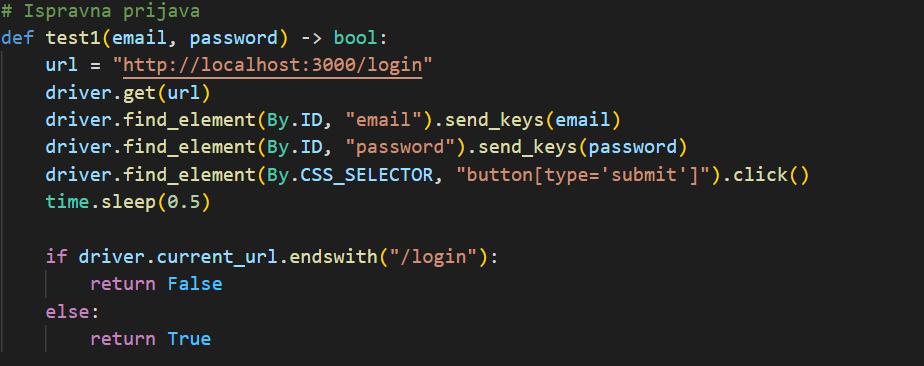
\includegraphics[scale=0.5]{dijagrami/test1.png}
    \centering
    \caption{prvi ispitni slučaj koji obrađuje ispravnu prijavu. Očekivani izlaz je uspješna prijava i preusmjeravanje.}

\end{figure}

\begin{figure}[htp]
    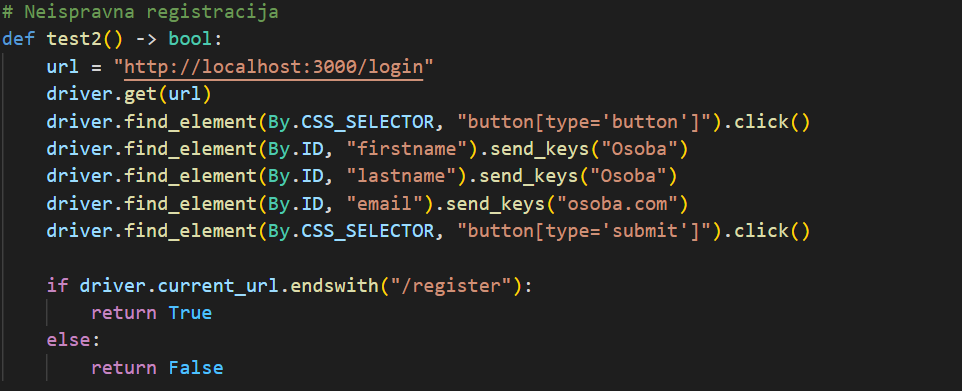
\includegraphics[scale=0.5]{dijagrami/test2.png}
    \centering
    \caption{drugi ispitni slučaj koji obrađuje neispravnu registraciju. Unosom maila u krivom formatu očekivani izlaz je neuspjela registracija.}
    
\end{figure}

\begin{figure}[htp]    
    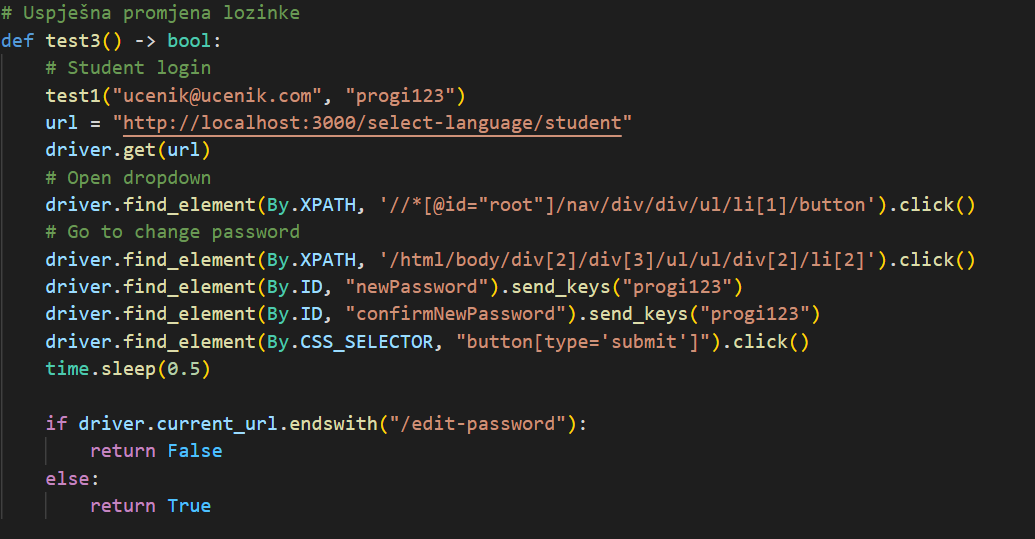
\includegraphics[scale=0.5]{dijagrami/test3.png}
    \centering
    \caption{treći ispitni slučaj koji obrađuje uspješnu promjenu lozinke. Preduvjet za promjenu lozinke je uspješna prijava u sustav kao student. Unosom podudarajućih lozinki očekivani izlaz je izmjena lozinke i preusmjeravanje.}

\end{figure}

\begin{figure}[htp]
    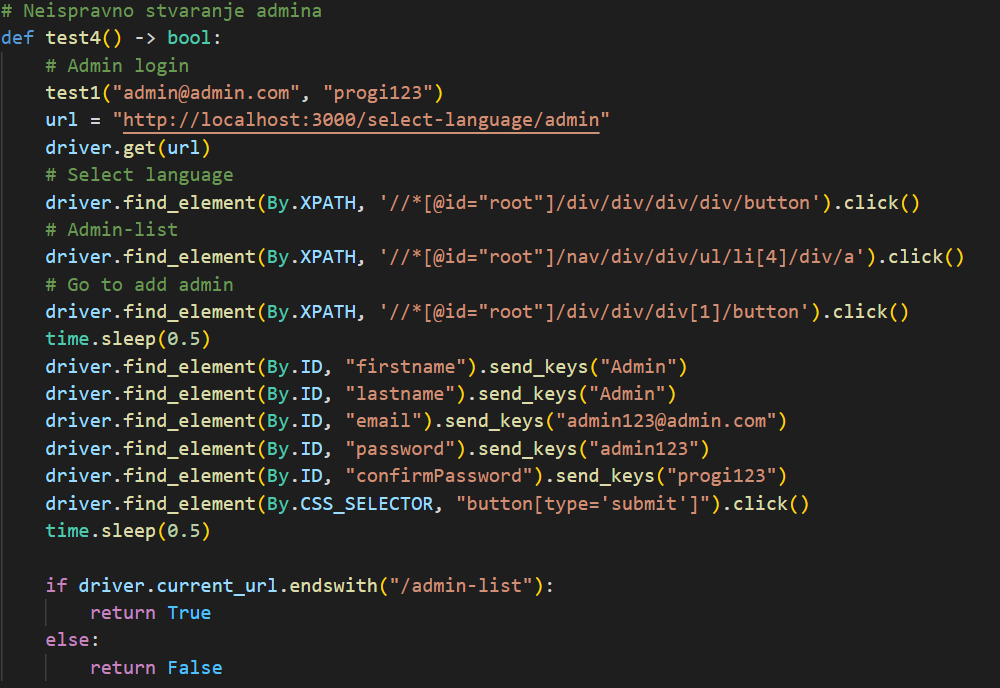
\includegraphics[scale=0.5]{dijagrami/test4.png}
    \centering
    \caption{četvrti ispitni slučaj koji obrađuje neispravno stvaranje admina. Preduvjet za stvaranje admina je uspješna prijava u sustav kao admin. Unosom nepodudarajućih lozinki u predložak, očekivani izlaz je neuspjela kreacija admina.}

\end{figure}

\begin{figure}[htp]
    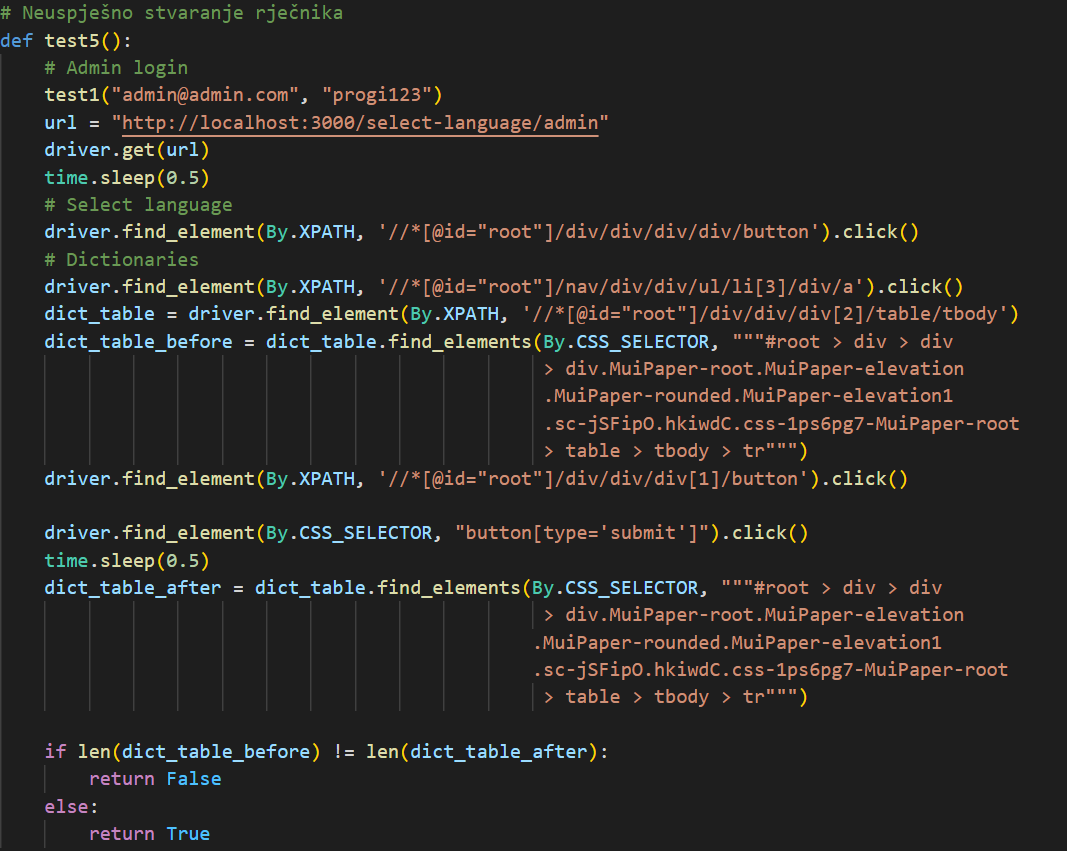
\includegraphics[scale=0.5]{dijagrami/test5.png}
    \centering
    \caption{peti ispitni slučaj koji obrađuje stvaranje rječnika s praznim imenom. Preduvjet za stvaranje rječnika je uspješna prijava u sustav kao admin. Bez unosa imena novog rječnika očekivani izlaz je nepromijenjeno stanje tablice rječnika u sustavu.}

\end{figure}

\begin{figure}[htp]
    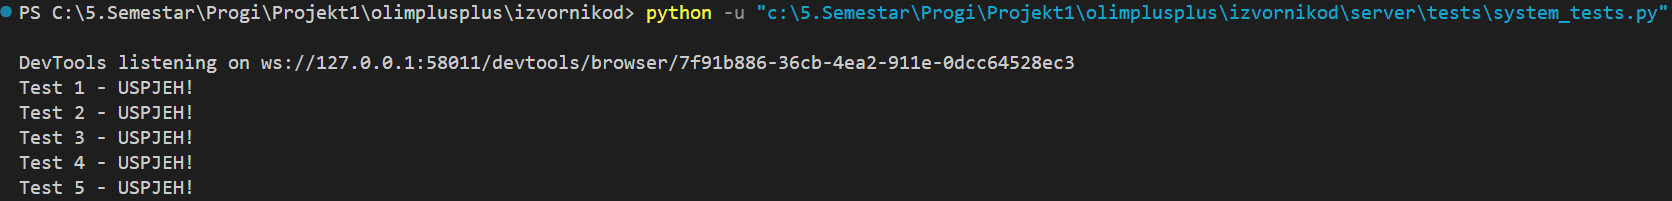
\includegraphics[scale=0.35]{dijagrami/terminal_screen.png}
    \centering
    \caption{terminal nakon pokretanja testova ispitivanja sustava.}
    
\end{figure}

\clearpage

\eject

		
		\section{Dijagram razmještaja}

        Aplikacija je organizirana u tri razine: klijentsku, serversku i podatkovnu. Klijentska razina izvršava se u web pregledniku koji pokreće React aplikaciju. Serverska razina pokreće se na odvojenom poslužitelju u Python 3.11.7 okruženju koji komunicira s PostgreSQL 15 bazom podataka puštenom u pogon na trećem računalu. Komunikacija između izvršnih okruženja odvija se protokolom HTTP.
			
		\begin{figure}[htp]
			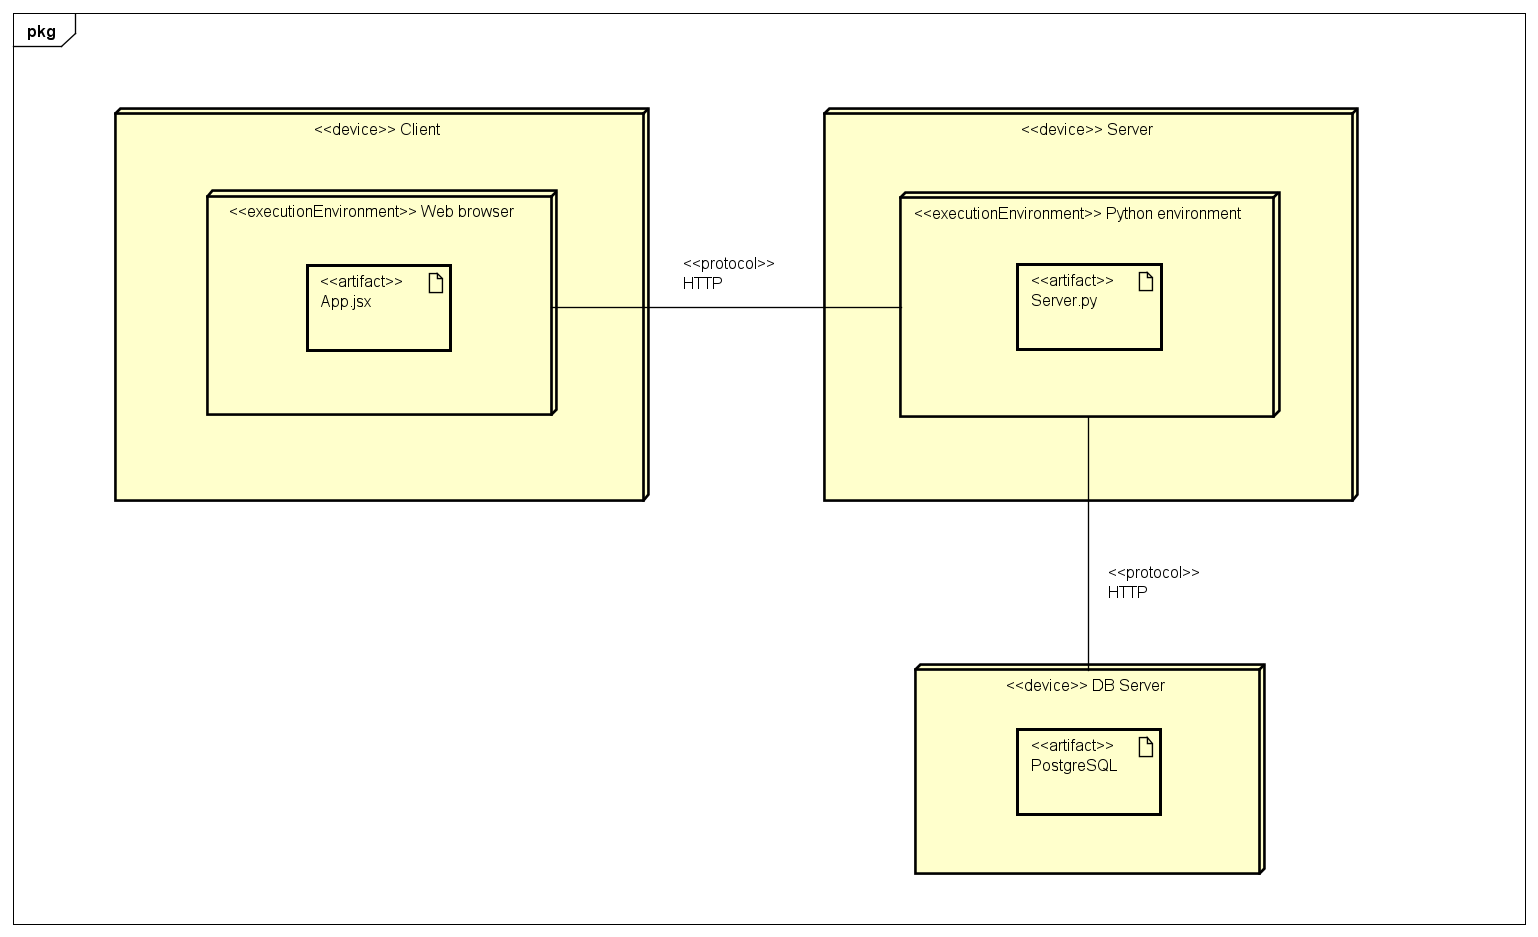
\includegraphics[scale=0.35]{dijagrami/DeploymentDiagram0.png}
			\centering
			\caption{Dijagram razmještaja}
		\end{figure}

        \eject
		
		\section{Upute za puštanje u pogon}

        Aplikaciju puštamo u pogon preko usluge \href{https://render.com/}{Render} koju povezujemo s repozitorijem na GitHubu. Ovakva konfiguracija omogućava nam da jednom postavljenu aplikaciju možemo automatski ponovno pustiti u pogon pushem na granu koju smo odabrali kao produkcijsku. Puštanje u pogon odvija se u tri faze.

        \subsection{Baza podataka}

        \begin{packed_item}

            \item Nakon registracije i prijave u servis Render odabiremo gumb \emph{New PostgreSQL} (Slika \ref{fig:dep-1})
            \item Bazu podataka konfiguriramo prema Slici \ref{fig:dep-2} i potvrdimo unos
            \item Nakon uspješnog puštanja u pogon, iz postavki kopiramo vanjski URL za pristup bazi (Slika \ref{fig:dep-3})
            \item Inicijalizaciju baze provodimo pomoću biblioteke Flask-Migrate. URL za pristup bazi pohranimo lokalno u varijablu okruženja na serverskom dijelu aplikacije. Izvršavanjem naredbe \emph{flask --app server db upgrade} u lokalnom okruženju izvršavaju se sve stvorene \emph{up} migracije i u produkcijskoj bazi stvaraju se sve potrebne tablice.
            
        \end{packed_item}

        \begin{figure}[htp]
			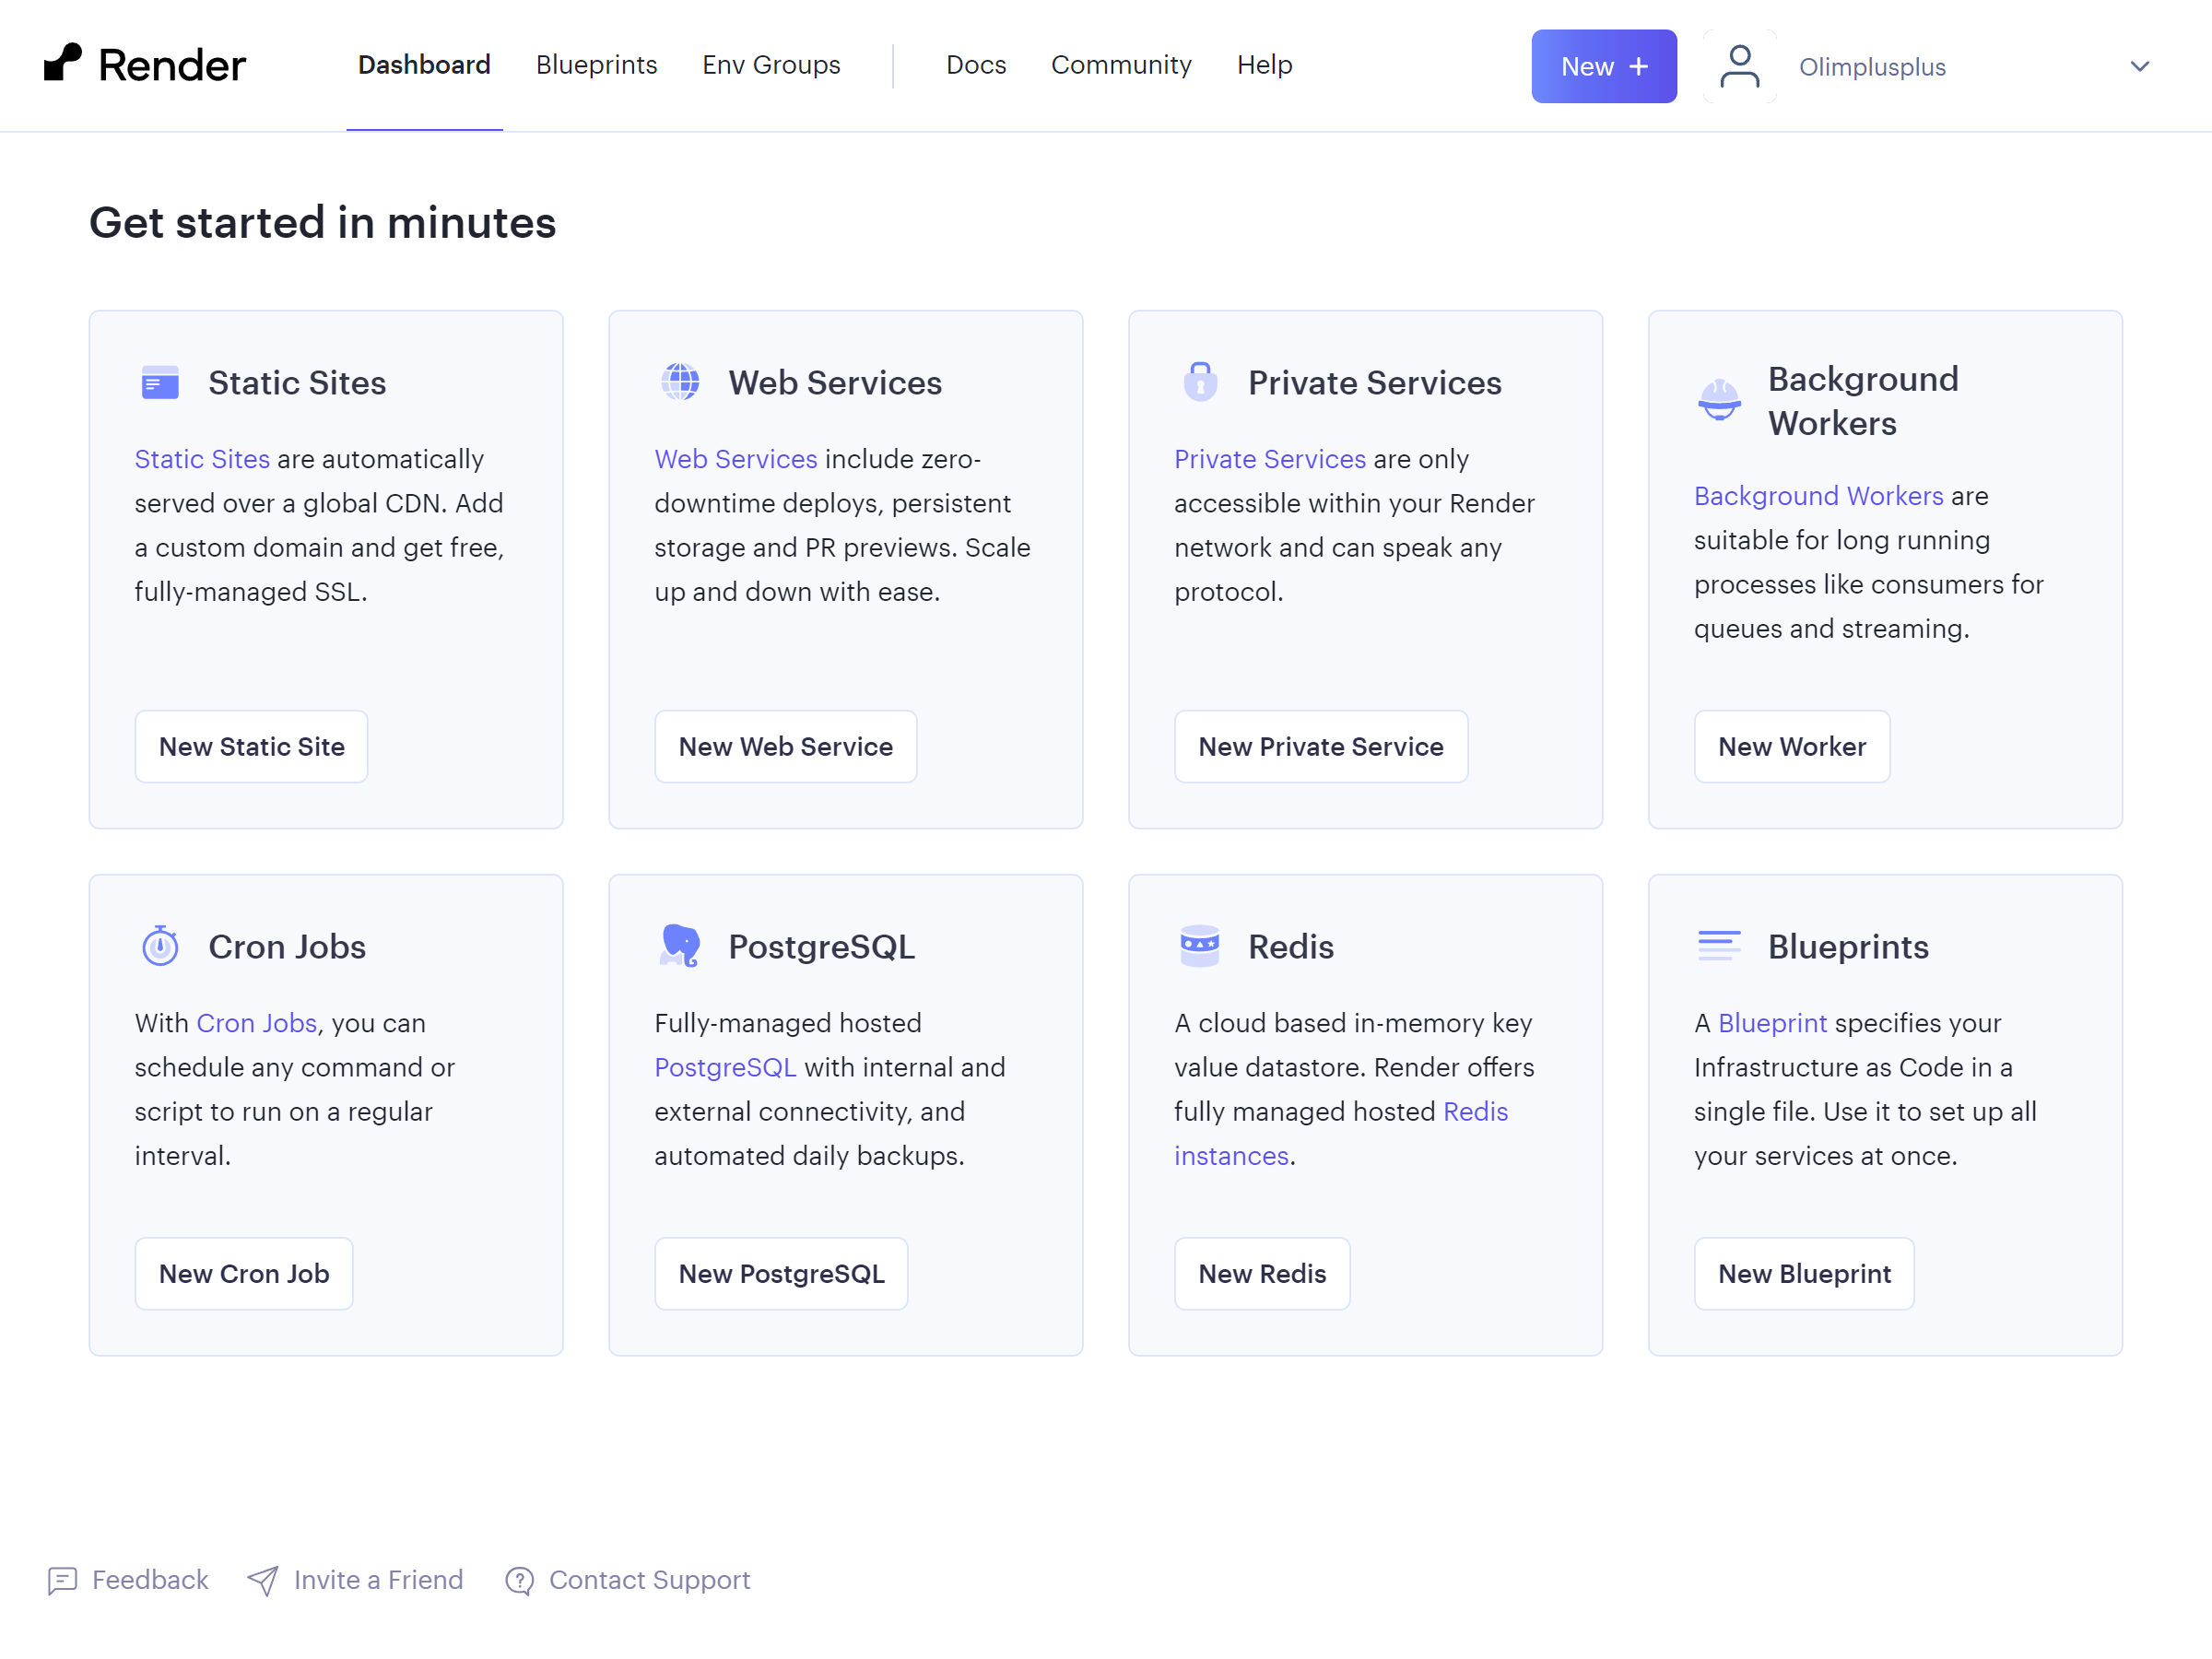
\includegraphics[scale=0.17]{slike/deploy_1.png}
			\centering
			\caption{Dashboard zaslon nakon uspješne registracije}
            \label{fig:dep-1}
		\end{figure}

        \begin{figure}[htp]
			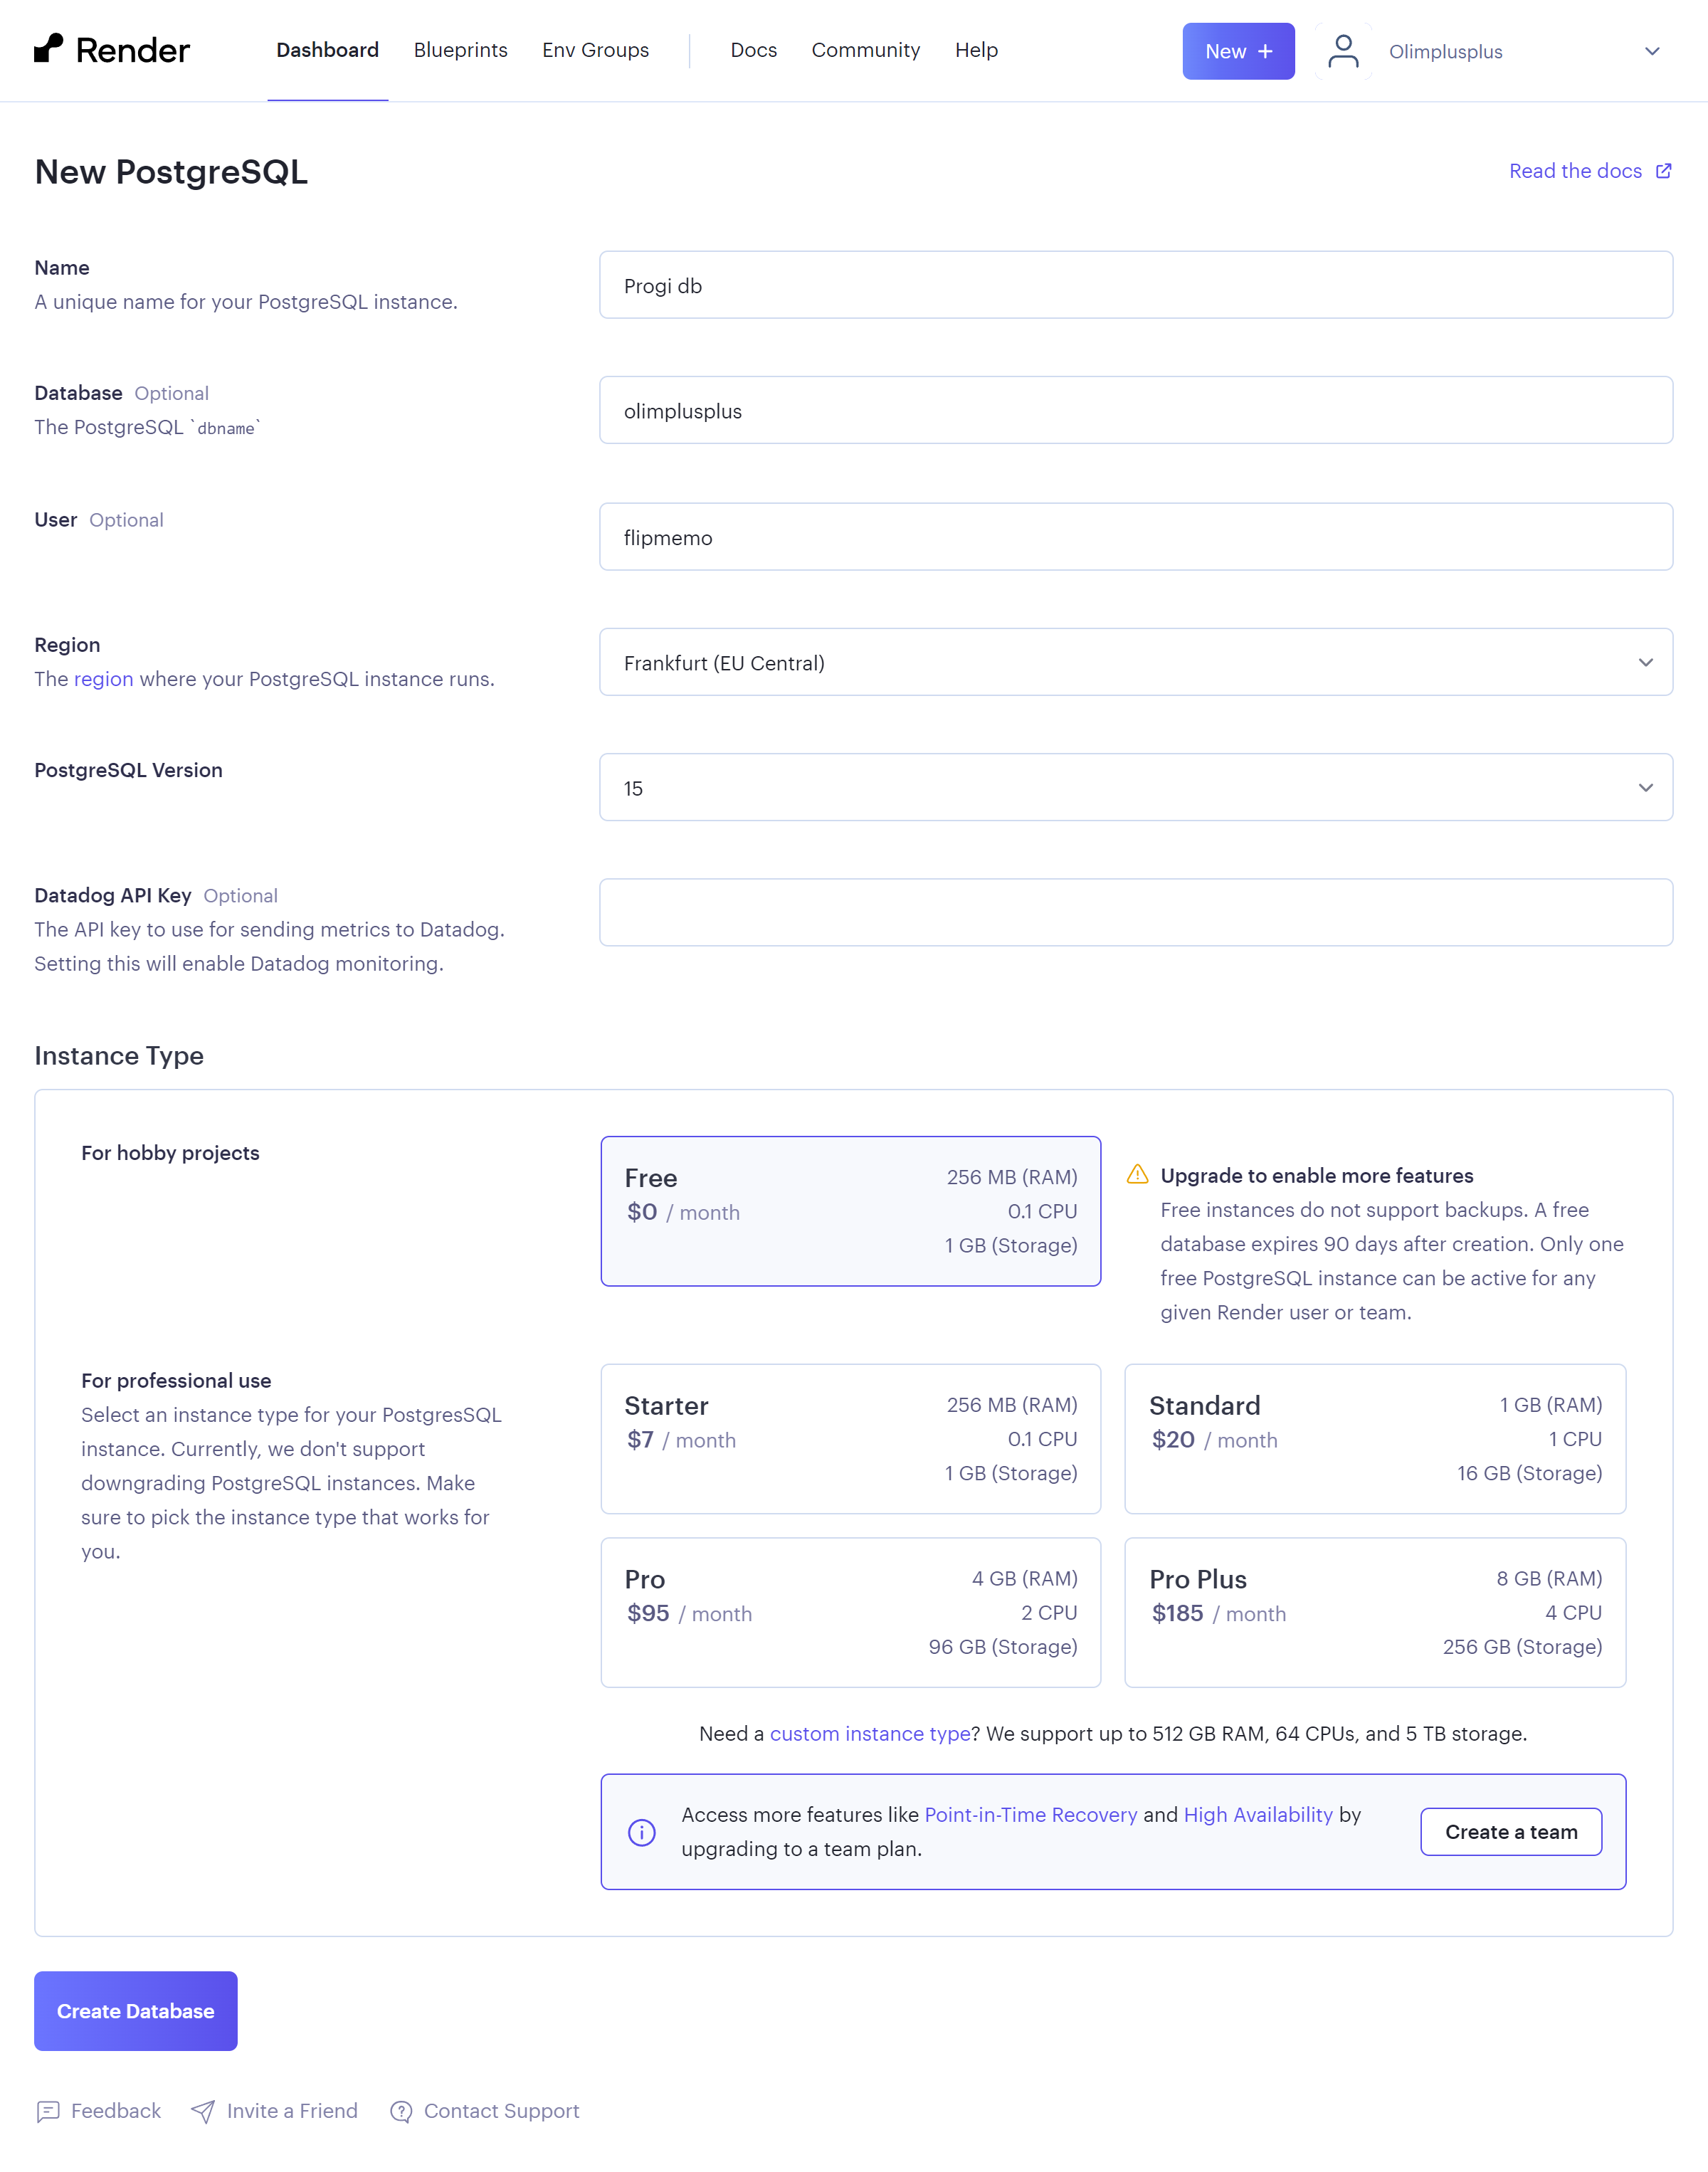
\includegraphics[scale=0.17]{slike/deploy_2.png}
			\centering
			\caption{Konfiguracija baze podataka}
            \label{fig:dep-2}
		\end{figure}

        \begin{figure}[htp]
			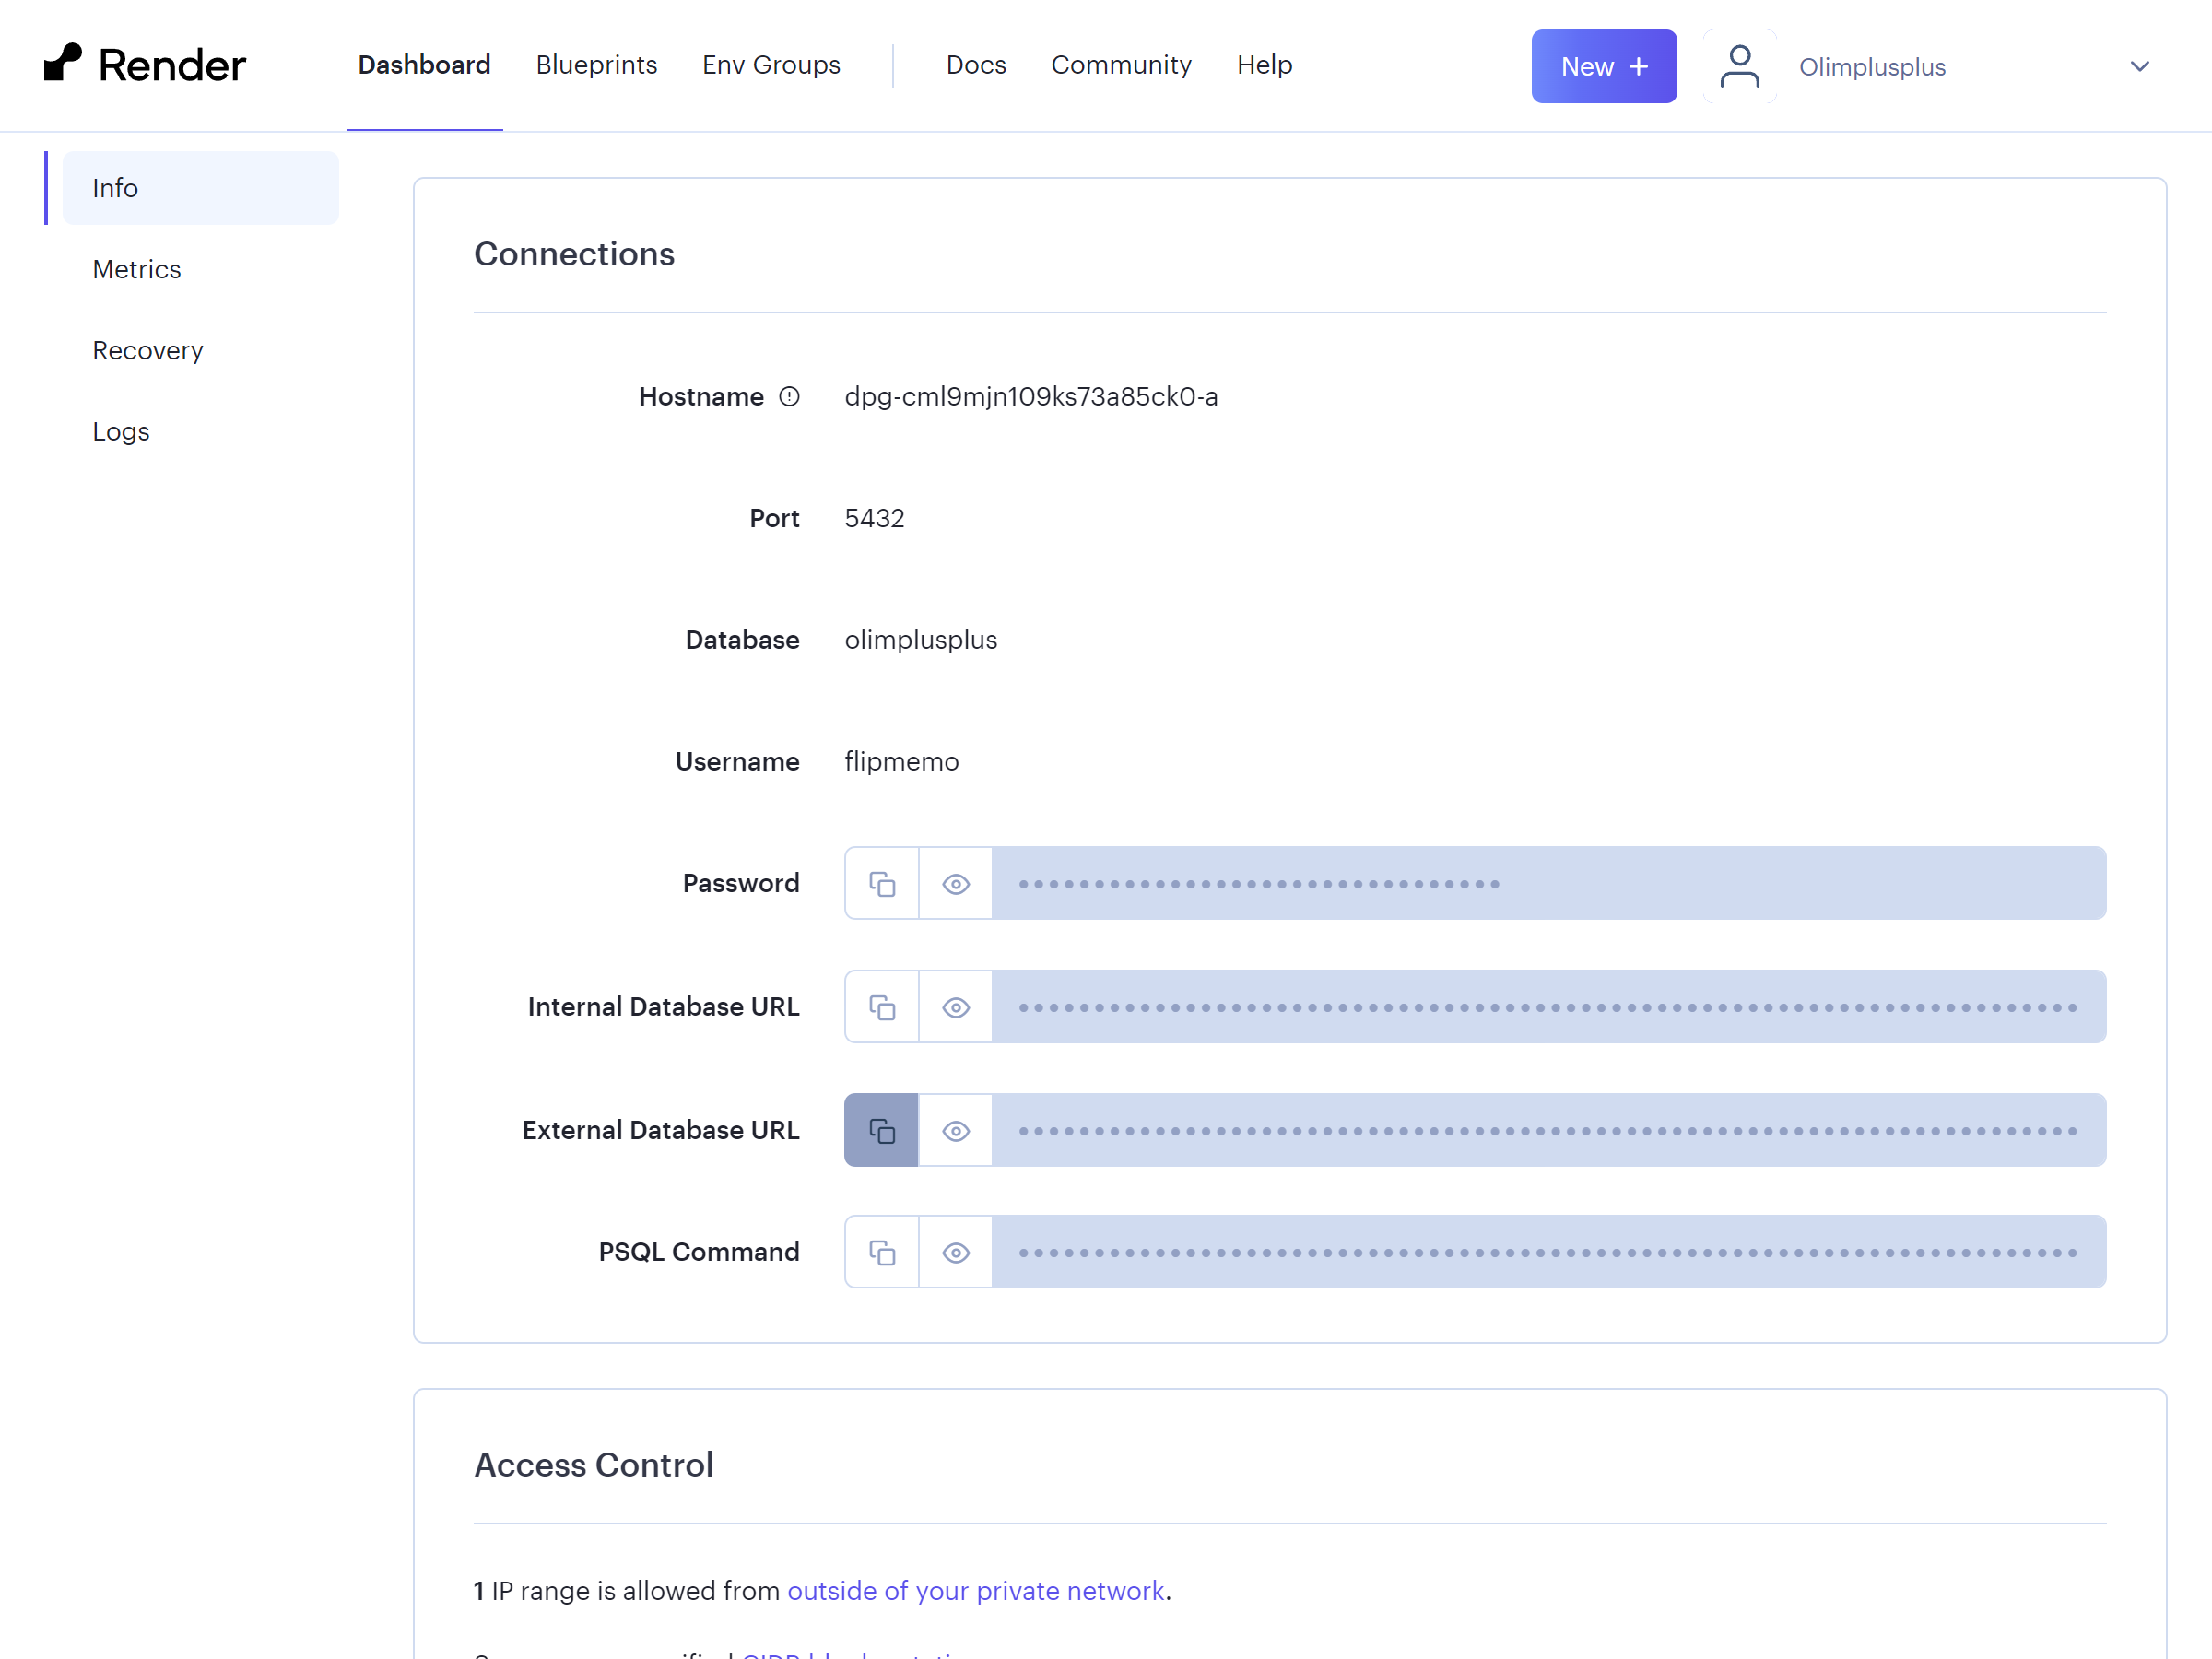
\includegraphics[scale=0.15]{slike/deploy_3.png}
			\centering
			\caption{Podaci za pristup bazi podataka}
            \label{fig:dep-3}
		\end{figure}

        \subsection{Poslužiteljski dio aplikacije}

        \begin{packed_item}

            \item Poslužiteljsku stranu puštamo u pogon kao web servis. Nakon odabira opcije \emph{Web Service} iz izbornika \emph{New} odabiremo opciju puštanja u pogon s GitHub repozitorija (Slika \ref{fig:dep-4}).
            \item Render povežemo s GitHub računom (Slika \ref{fig:dep-5}). Nakon uspješnog povezivanja moći ćete odabrati repozitorij kojeg želite pustiti u pogon (Slika \ref{fig:dep-6}).
            \item Web servis konfiguriramo prema slici Slika \ref{fig:dep-7} i potvrdimo unos.
            \item U postavkama stvorenog servisa pod odjeljkom \emph{Environments} trebamo stvoriti novu datoteku u koju ćemo spremiti sve potrebne varijable okruženja za pokretanje aplikacije, uključujući i URL za pristup bazi podataka (Slika \ref{fig:dep-9}).
            
        \end{packed_item}

        \begin{figure}[htp]
			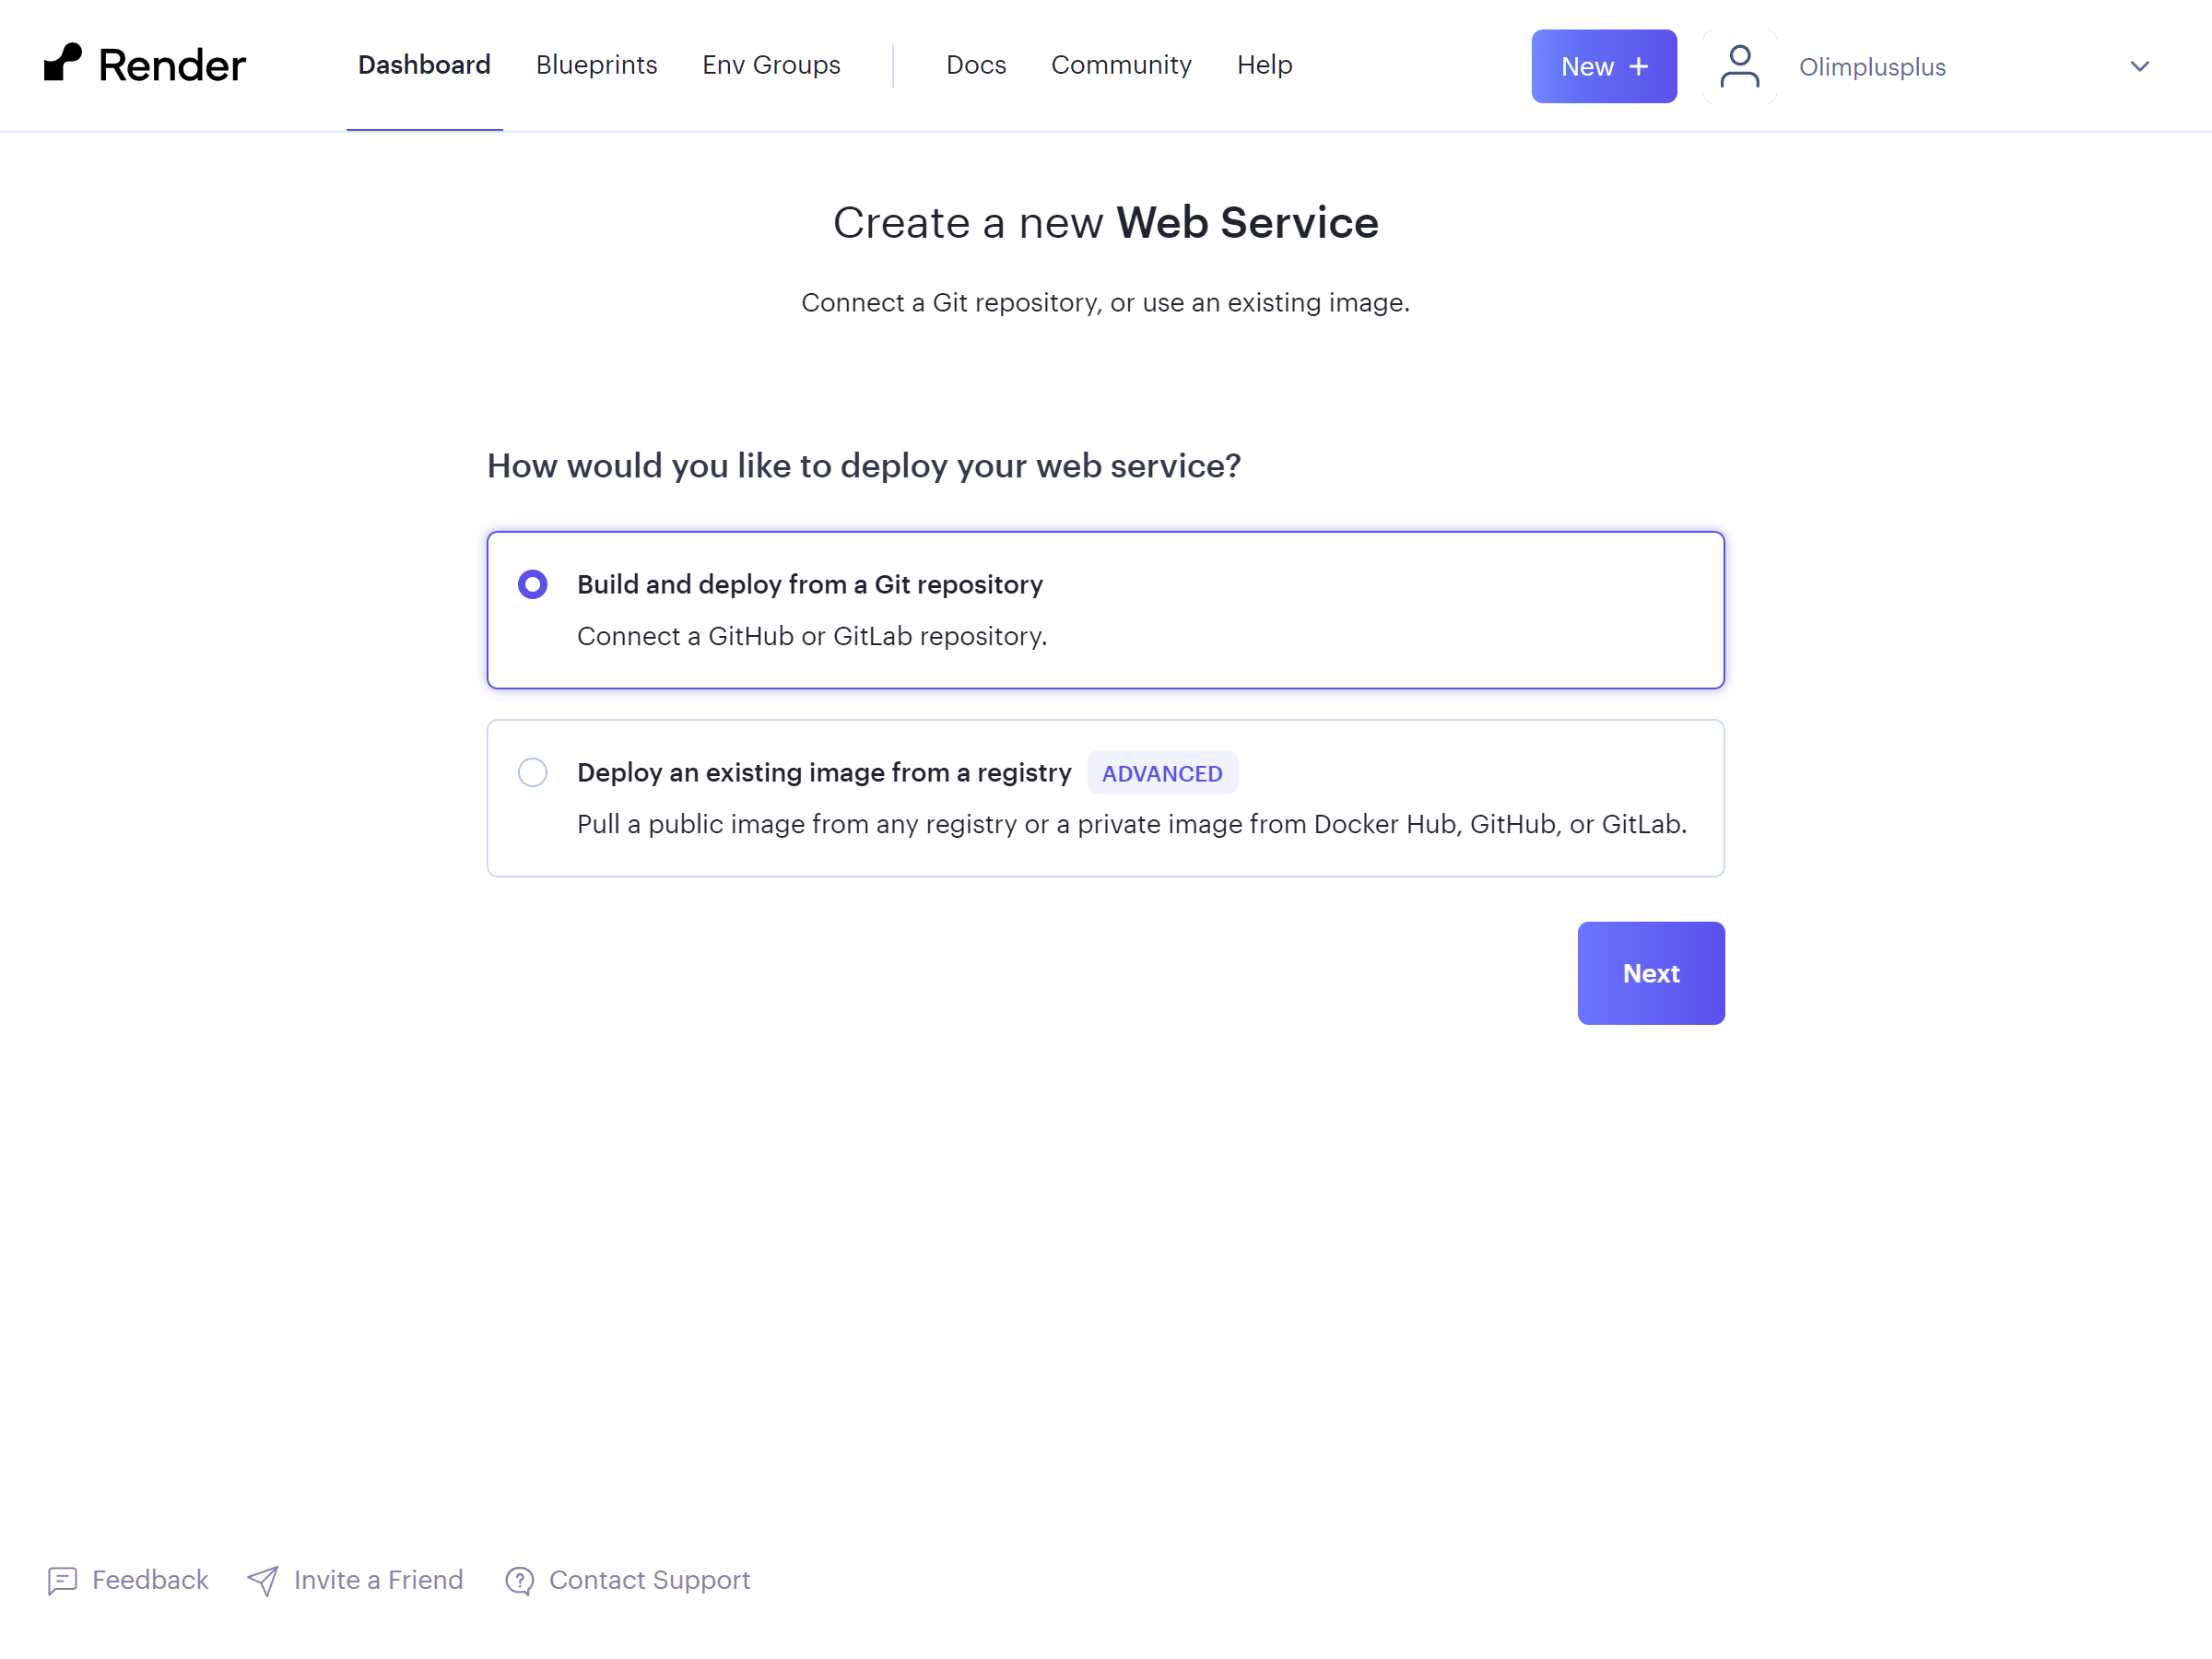
\includegraphics[scale=0.15]{slike/deploy_4.png}
			\centering
			\caption{Stvaranje web servisa}
            \label{fig:dep-4}
		\end{figure}

        \begin{figure}[htp]
			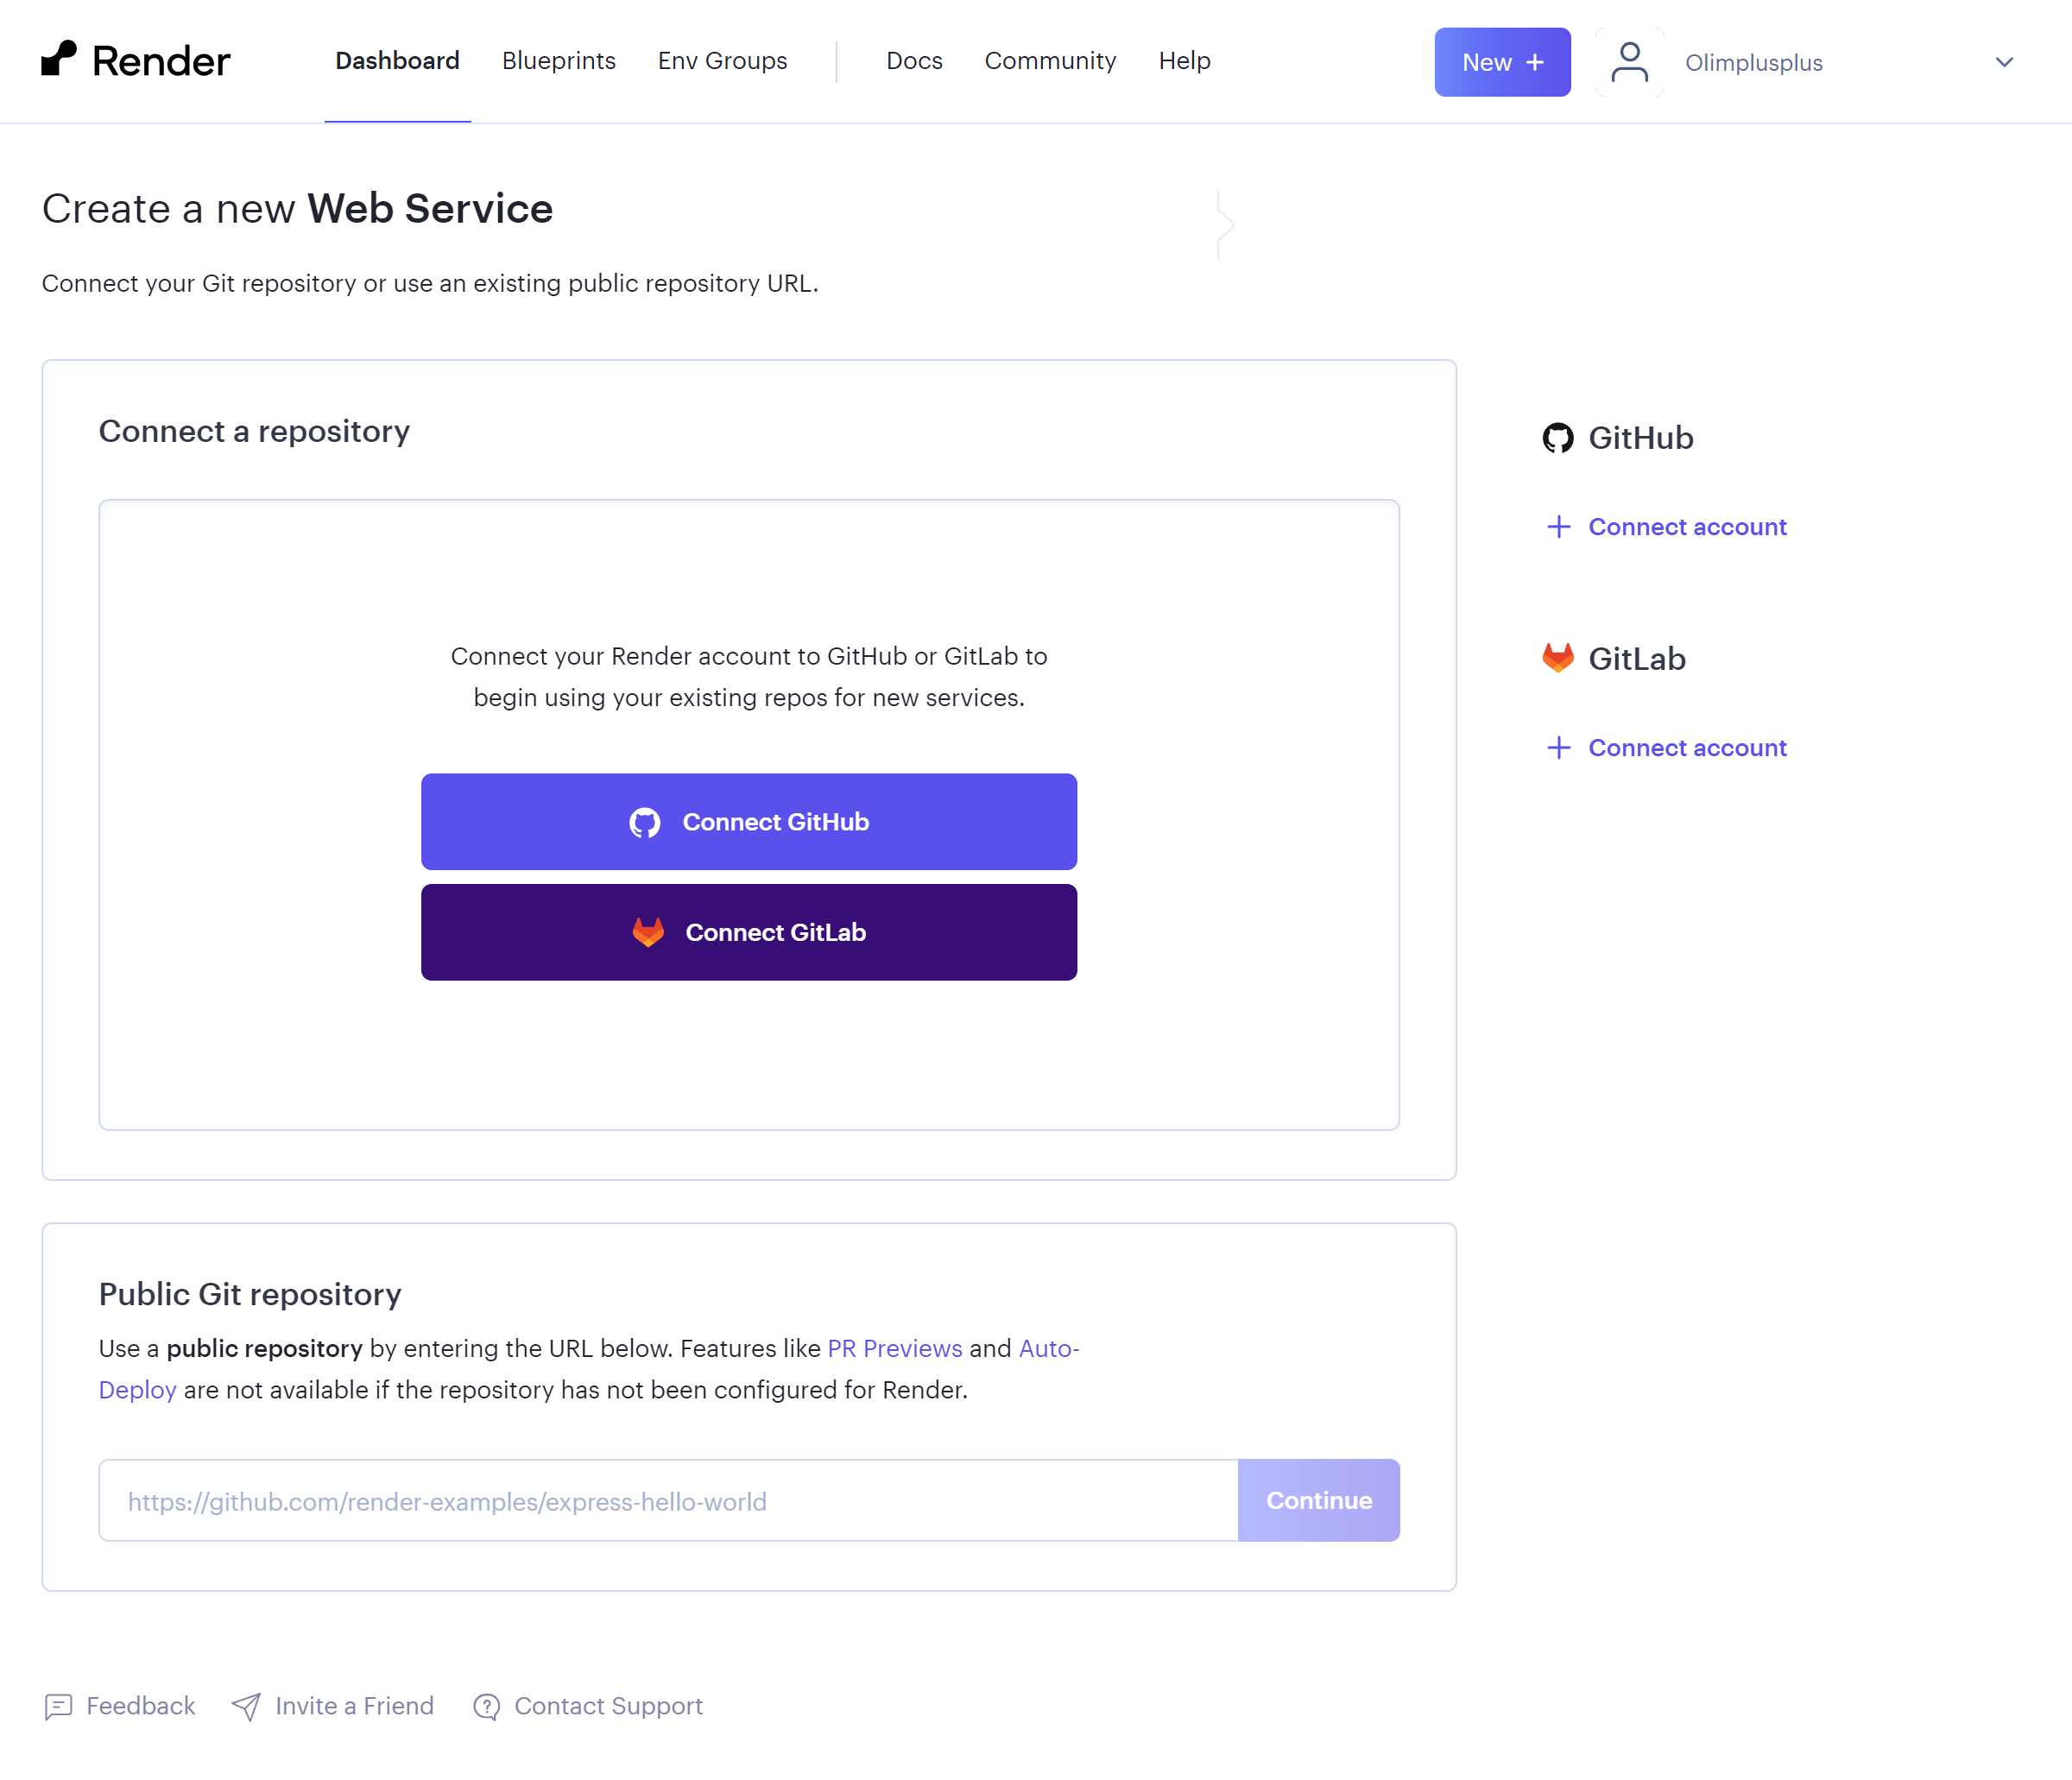
\includegraphics[scale=0.17]{slike/deploy_5.png}
			\centering
			\caption{Sučelje bez povezanog GitHub računa}
            \label{fig:dep-5}
		\end{figure}

        \begin{figure}[htp]
			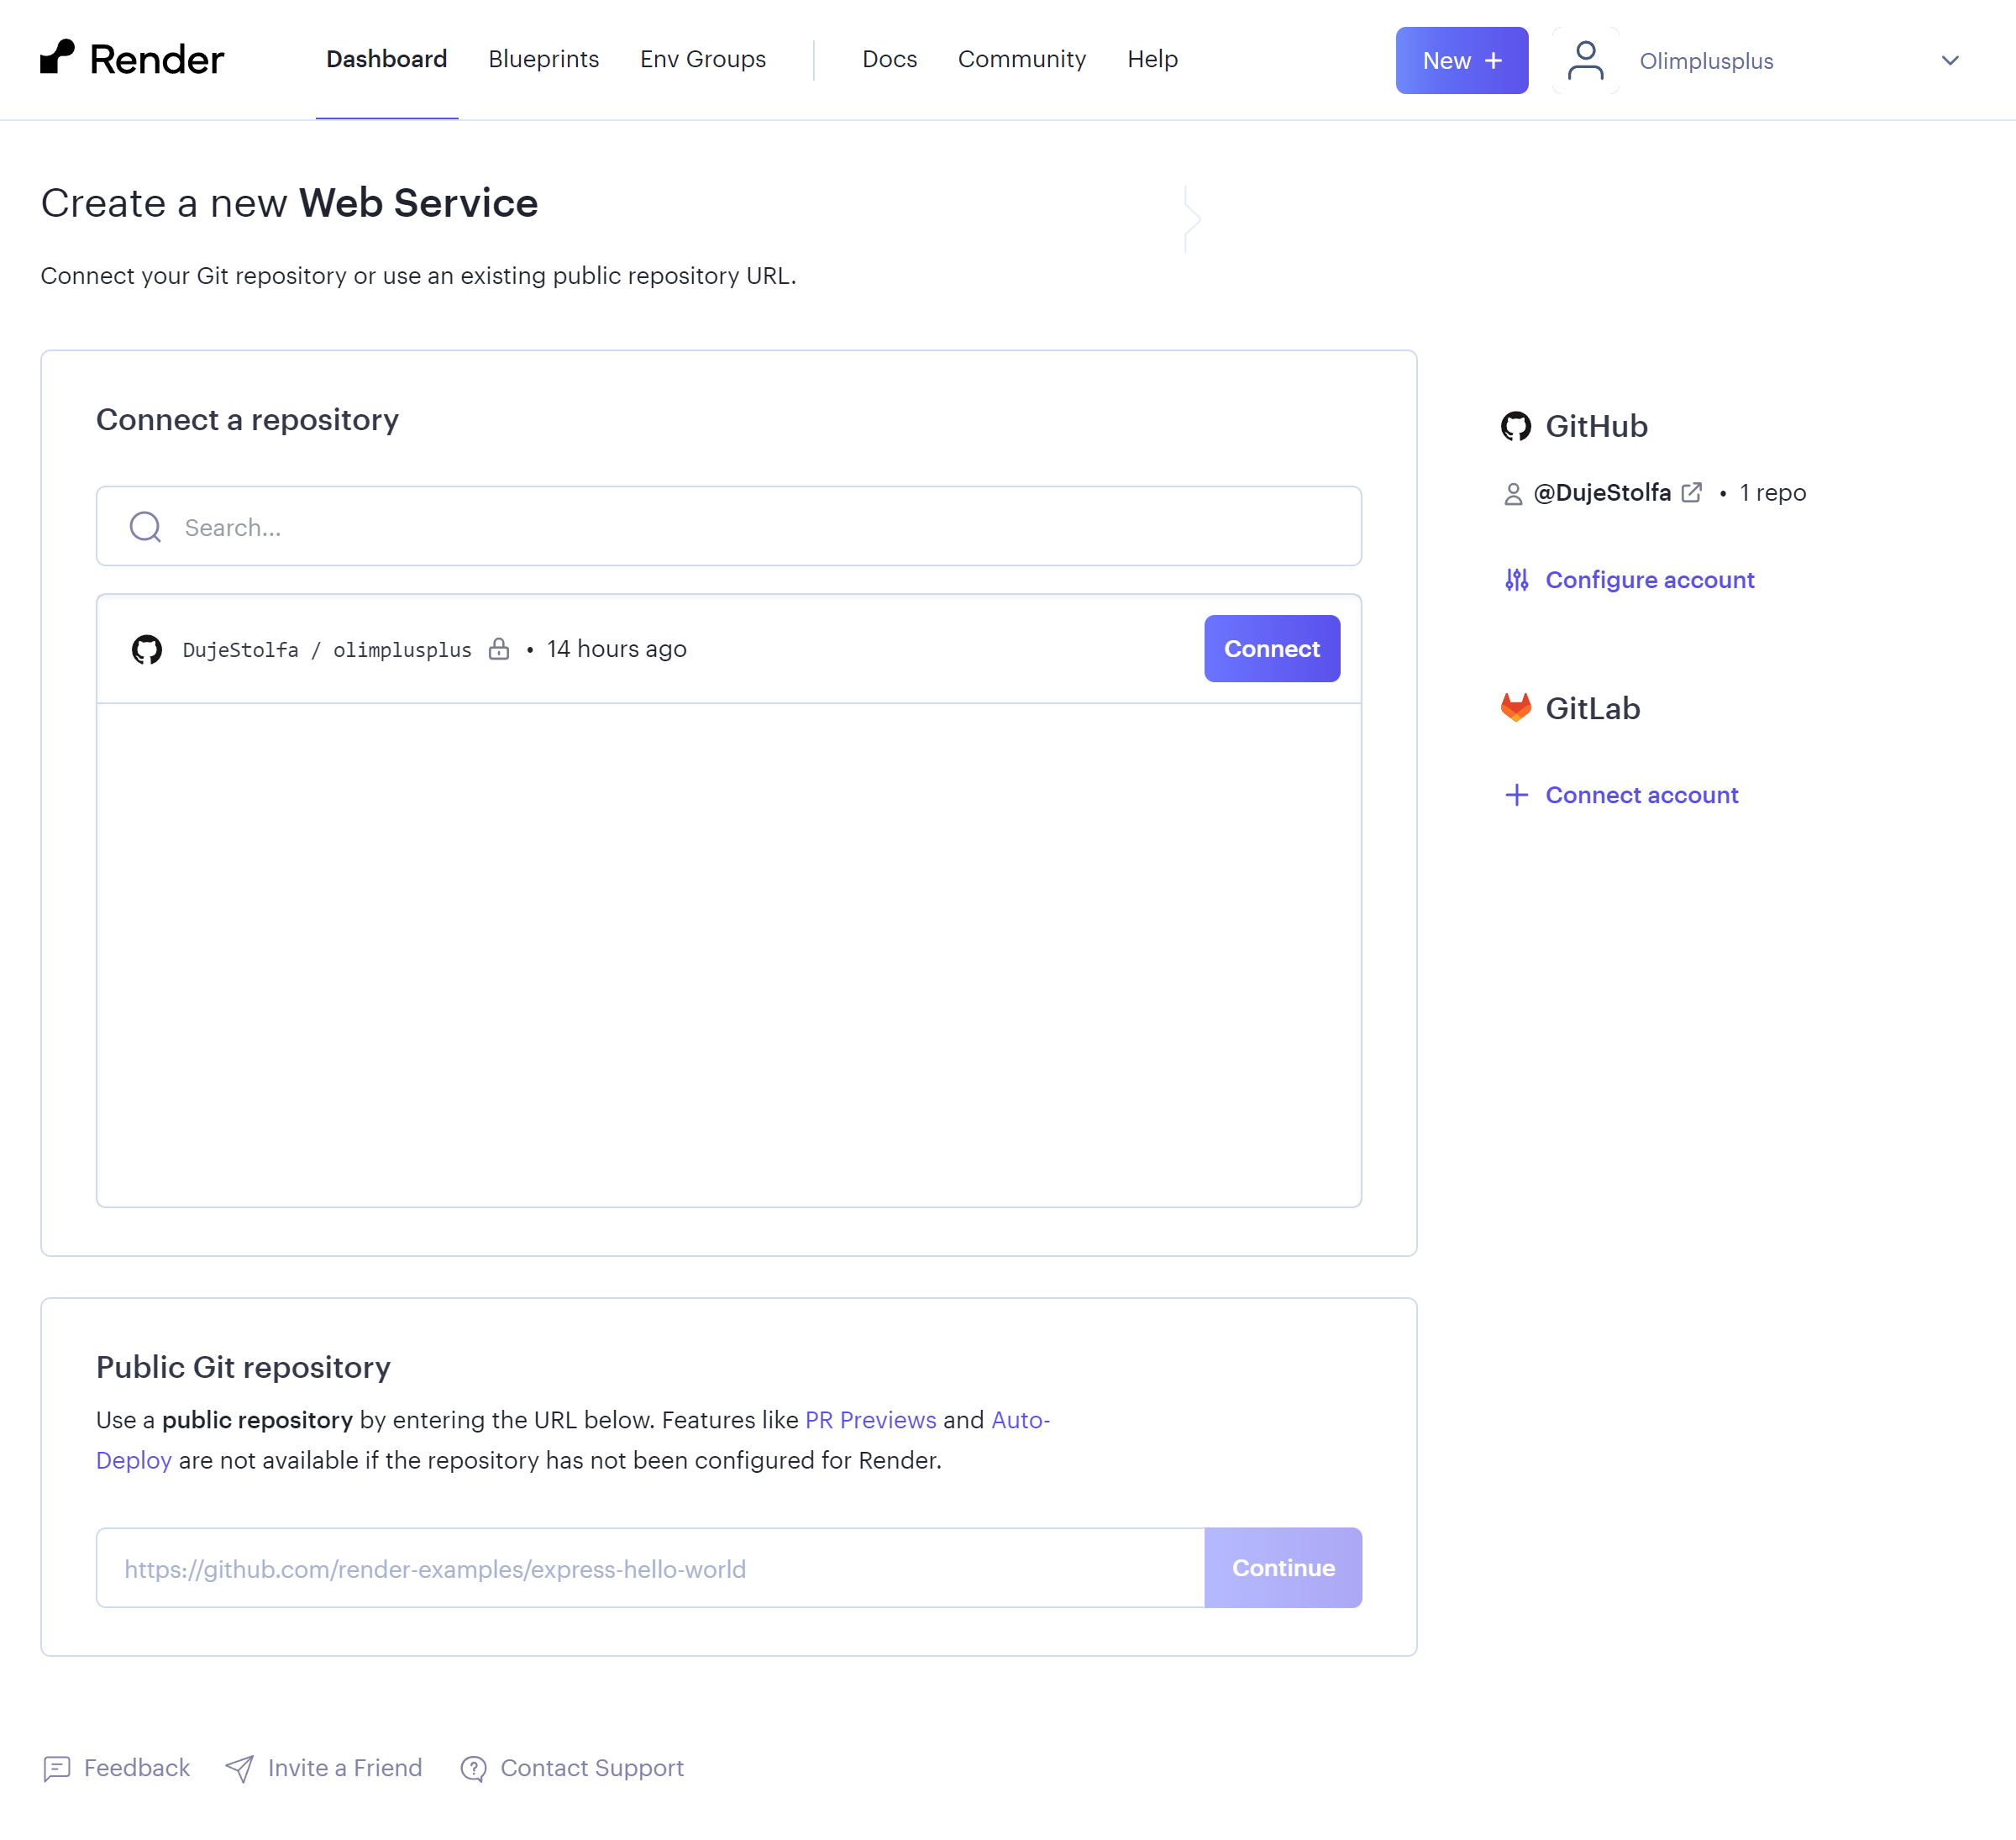
\includegraphics[scale=0.17]{slike/deploy_6.png}
			\centering
			\caption{Uspješno povezan GitHub račun}
            \label{fig:dep-6}
		\end{figure}

        \begin{figure}[htp]
			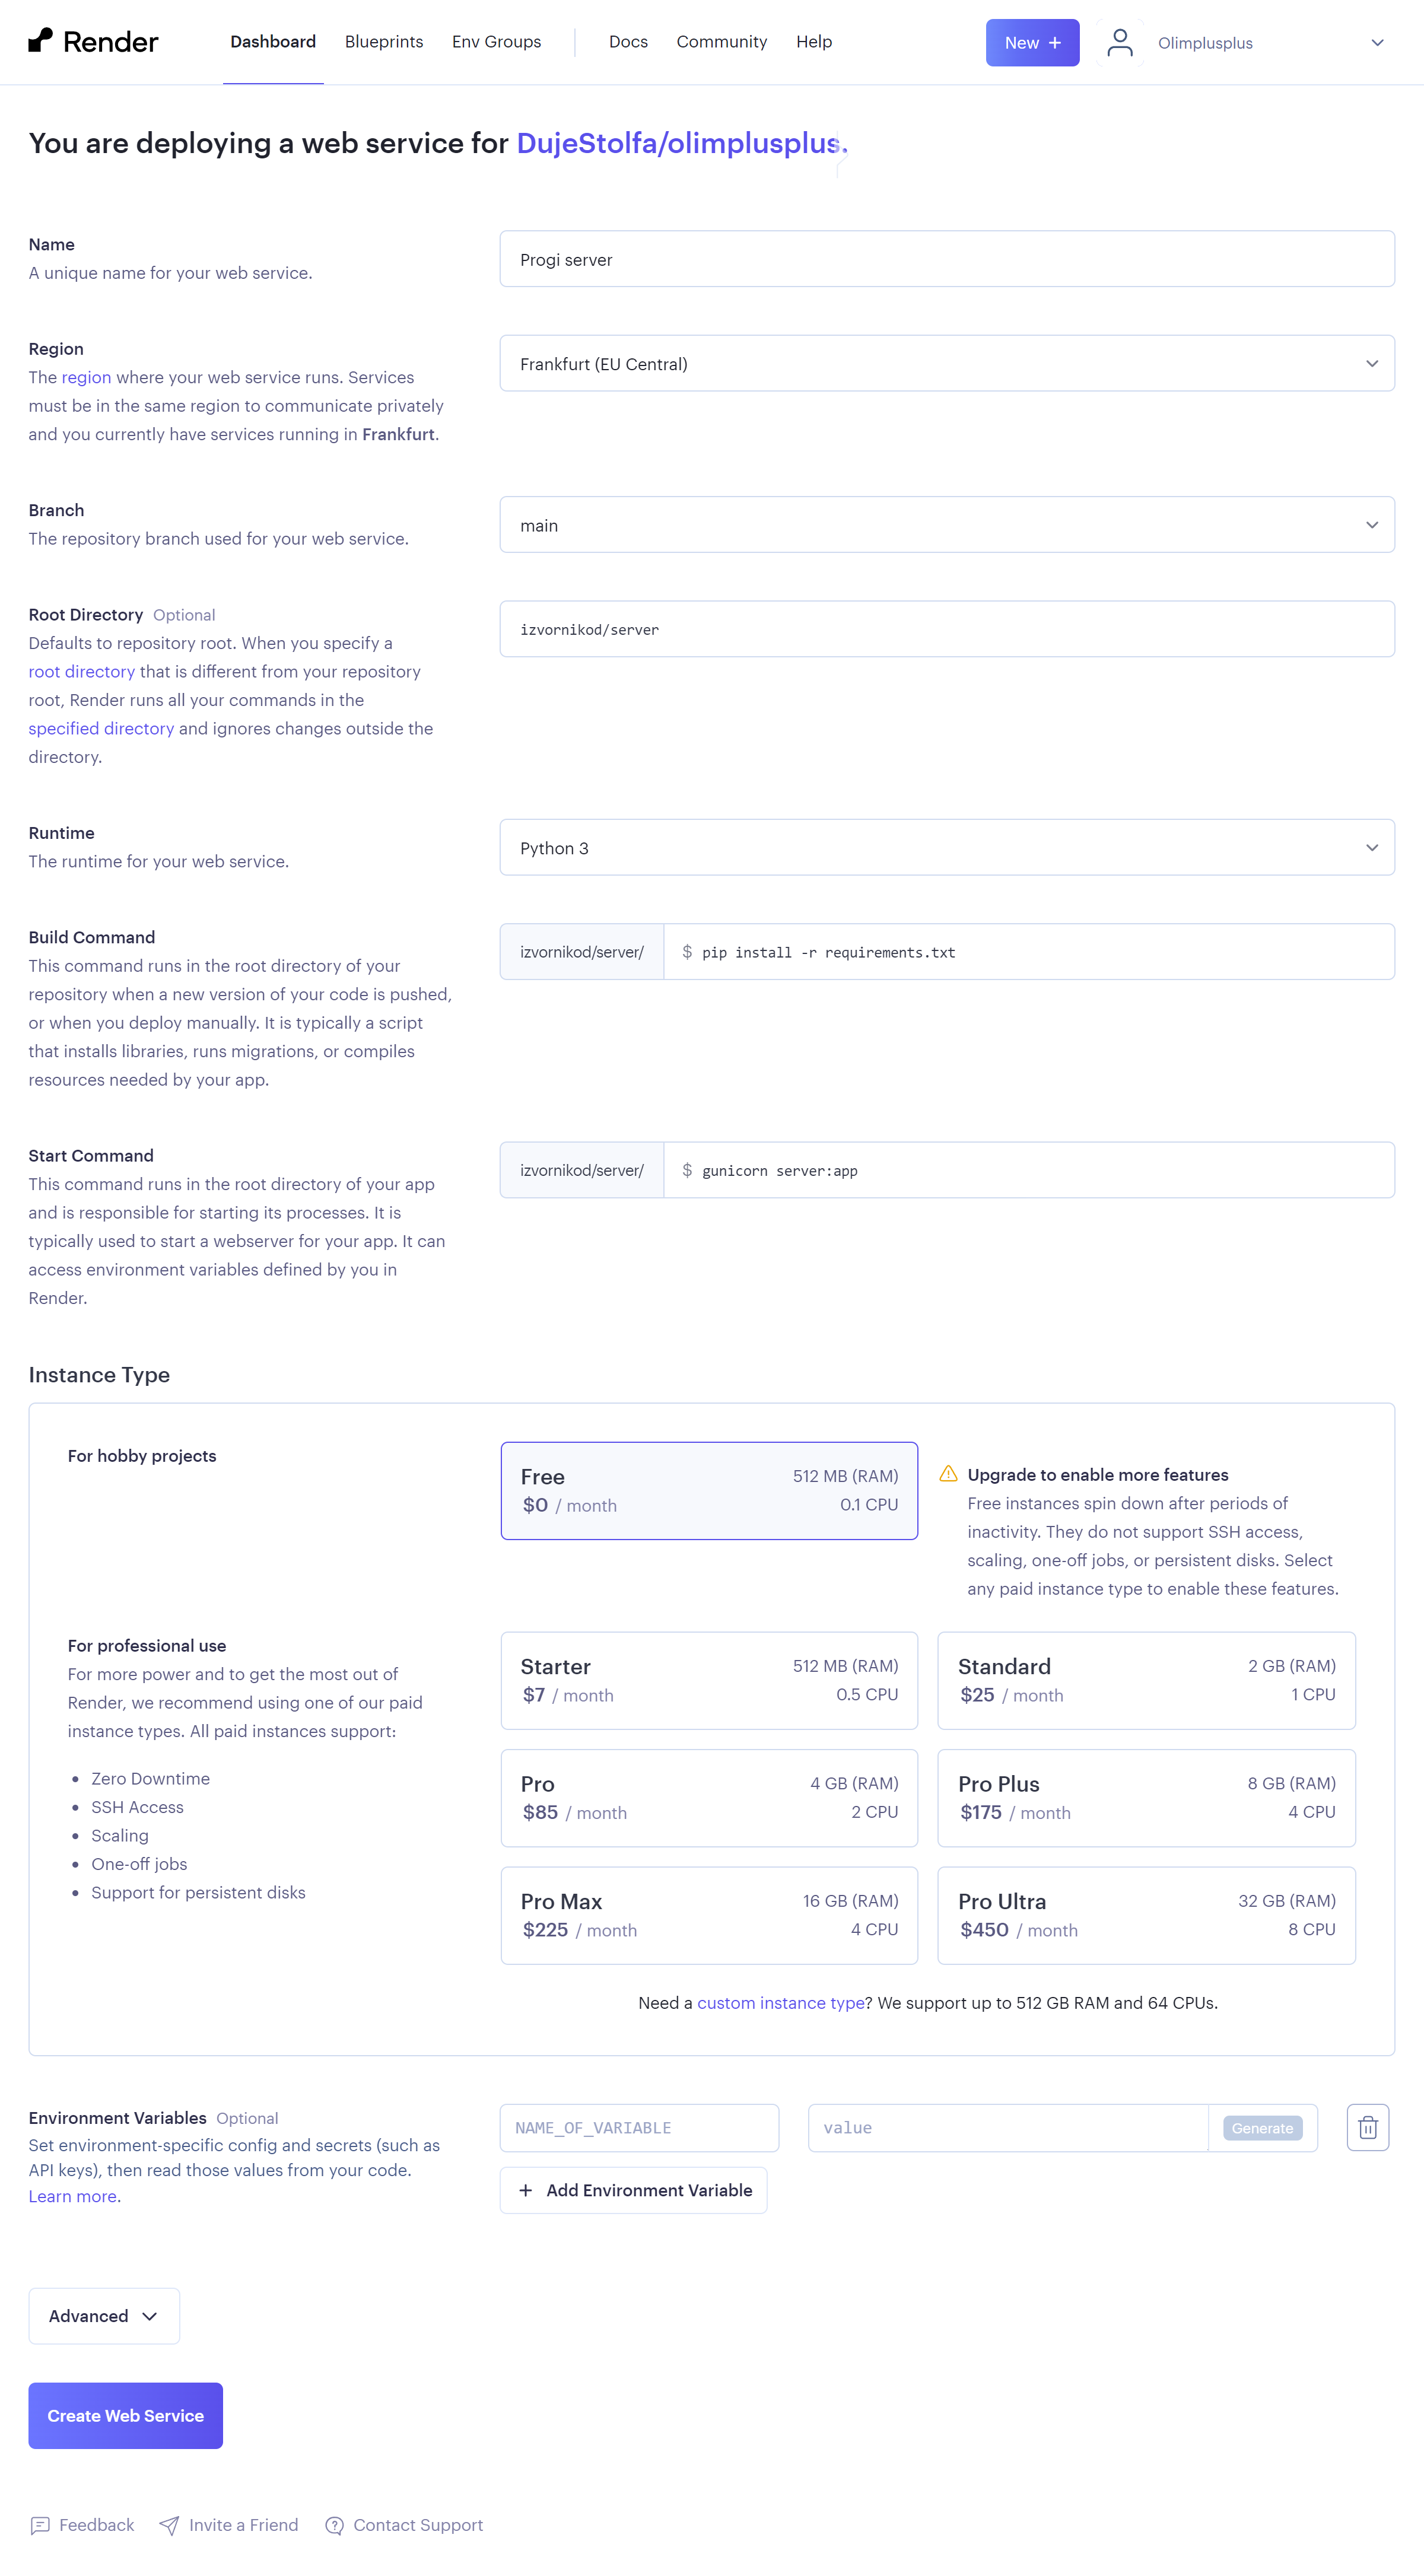
\includegraphics[scale=0.14]{slike/deploy_7.png}
			\centering
			\caption{Konfiguracija serverskog dijela aplikacije}
            \label{fig:dep-7}
		\end{figure}

        \begin{figure}[htp]
			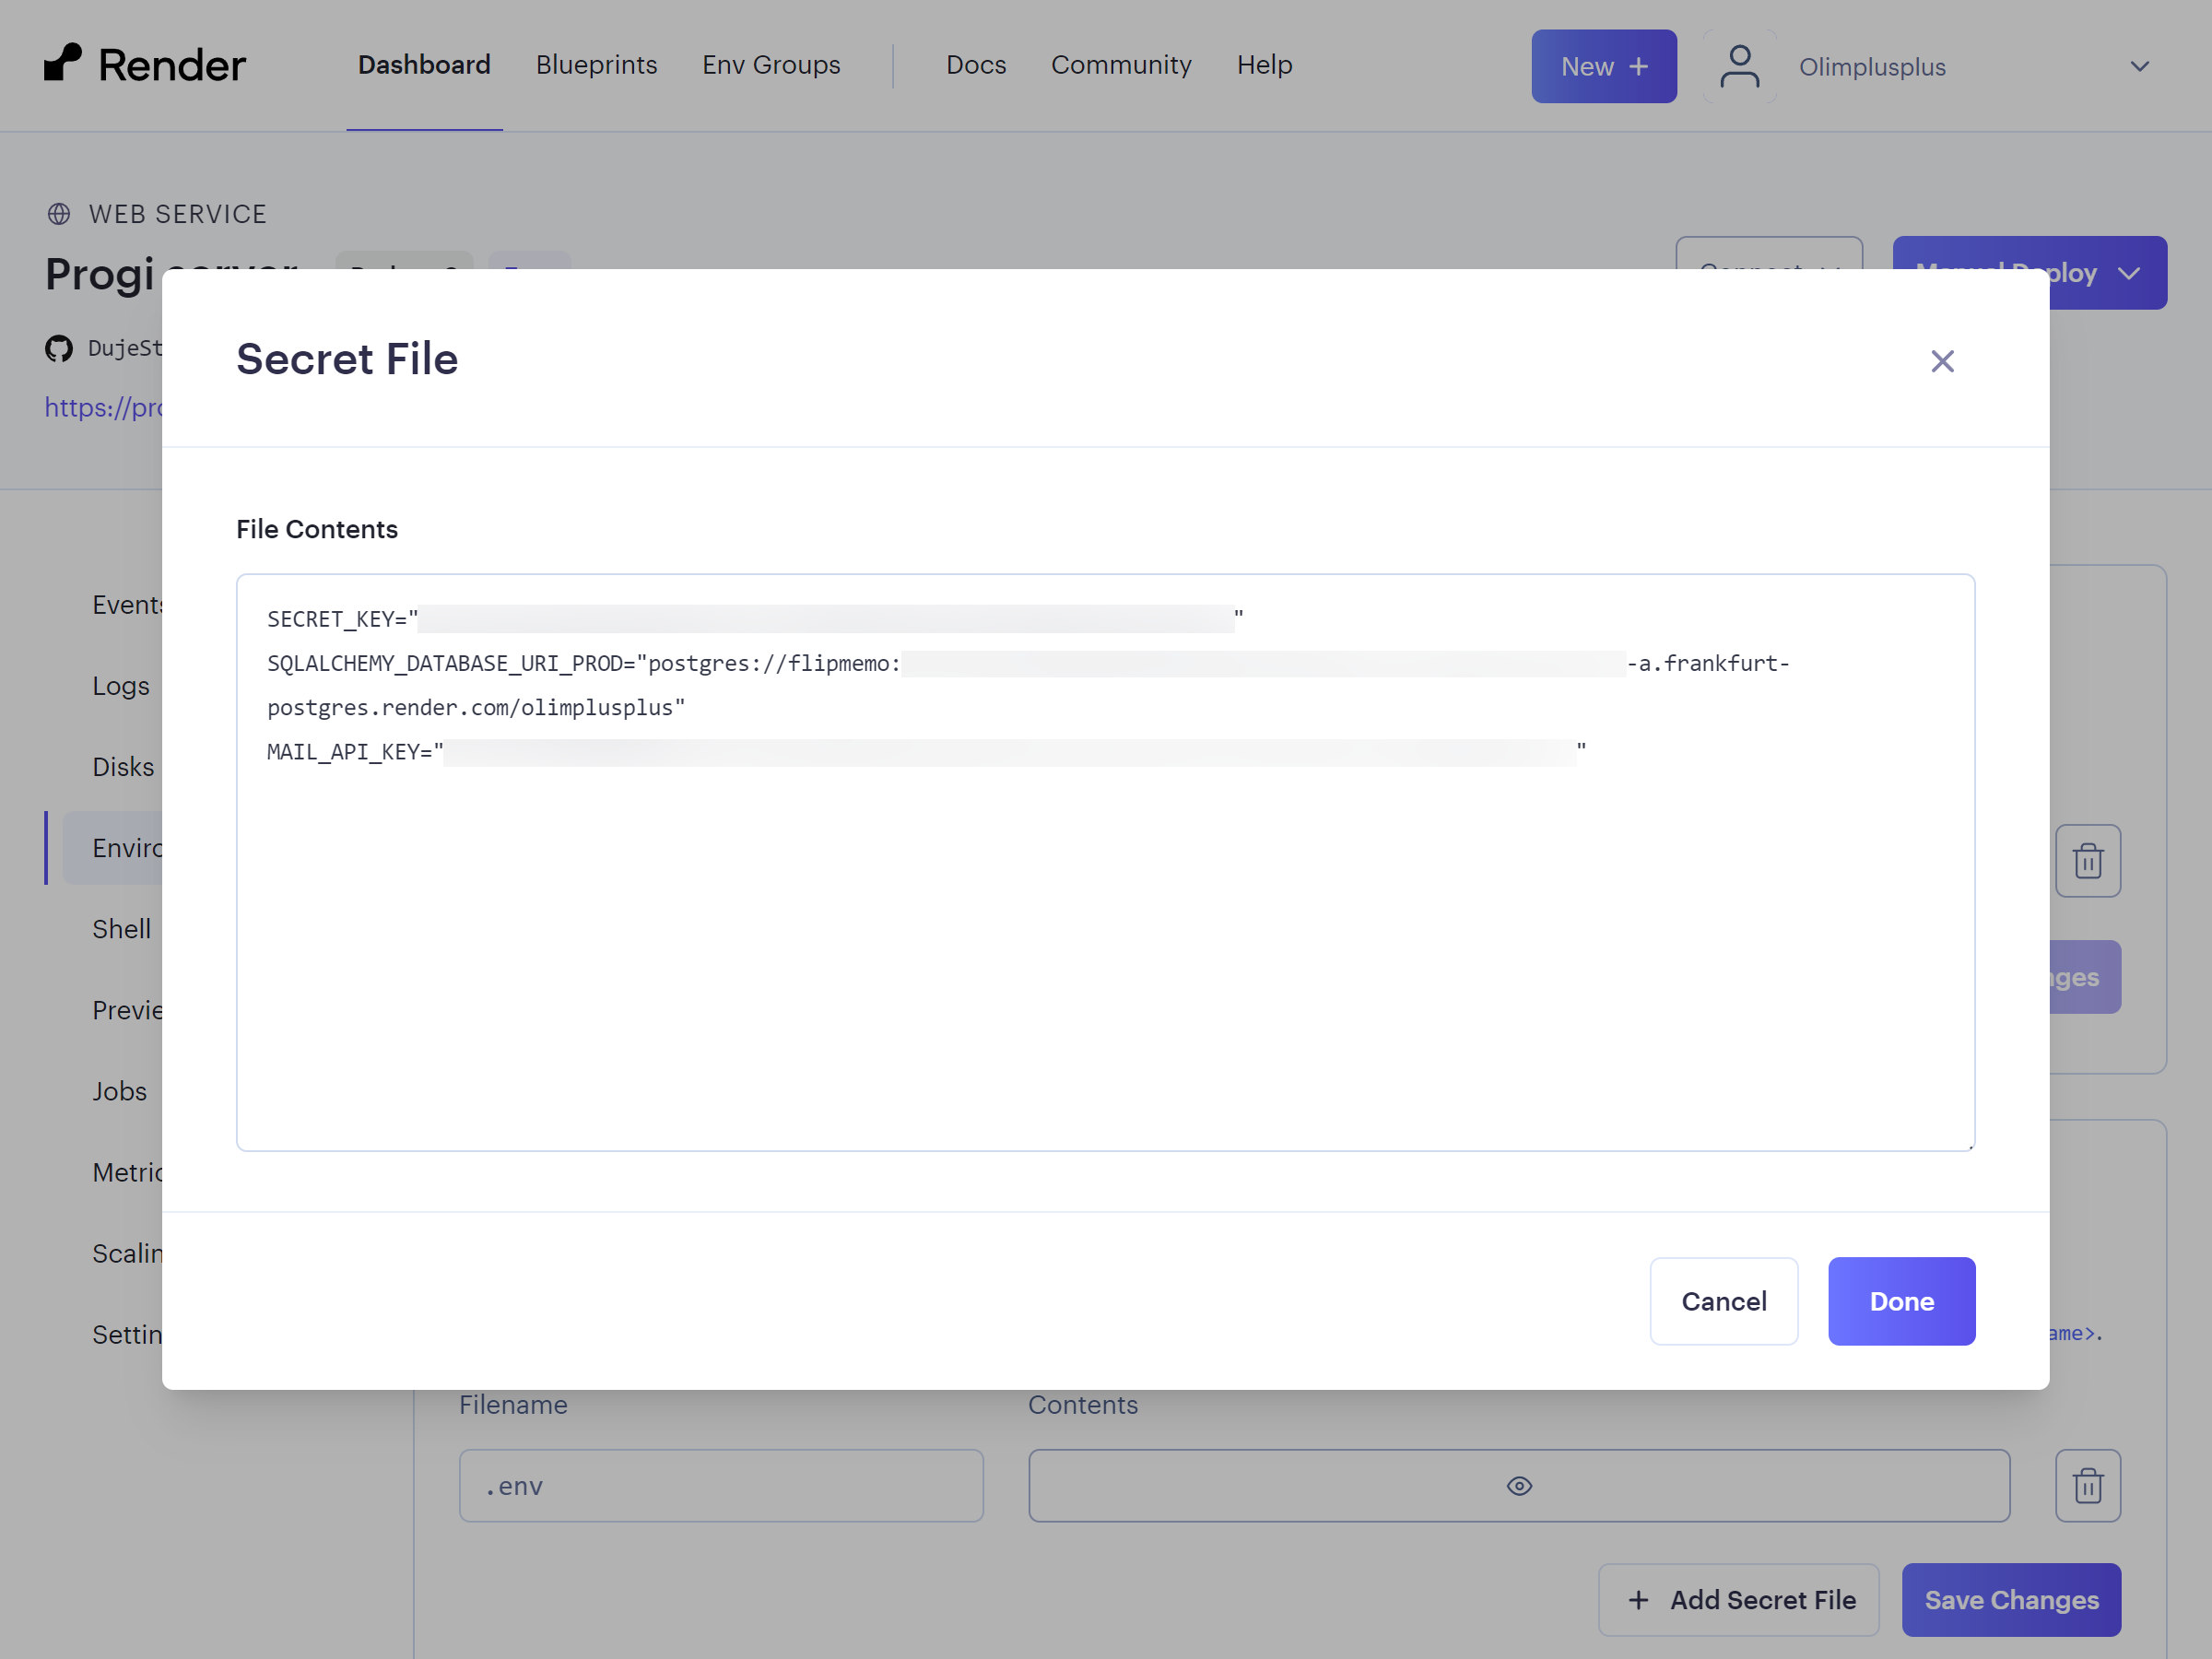
\includegraphics[scale=0.17]{slike/deploy_9.png}
			\centering
			\caption{Dodavanje varijabli okruženja na backend}
            \label{fig:dep-9}
		\end{figure}

        \eject

        \subsection{Klijentski dio aplikacije}

        \begin{packed_item}

            \item Prije puštanja fontenda u pogon potrebno je proširiti datoteku \emph{tsconfig.json} prema Slici \ref{fig:dep-10-5} i promjene pushati na git.
            \item Ovaj dio aplikacije također puštamo u pogon kao web servis i konfiguriramo ga prema Slici \ref{fig:dep-10} .
            
        \end{packed_item}

        Nakon navedenih koraka sve tri razine aplikacije trebale bi biti uspješno puštene u pogon (Slika \ref{fig:dep-11}).

        \begin{figure}[htp]
			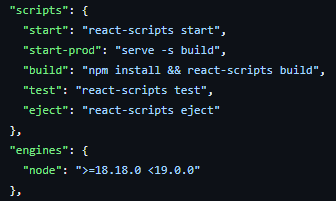
\includegraphics[scale=1]{slike/deploy_10_5.png}
			\centering
			\caption{Produkcijska konfiguracija React aplikacije}
            \label{fig:dep-10-5}
		\end{figure}

        \begin{figure}[htp]
			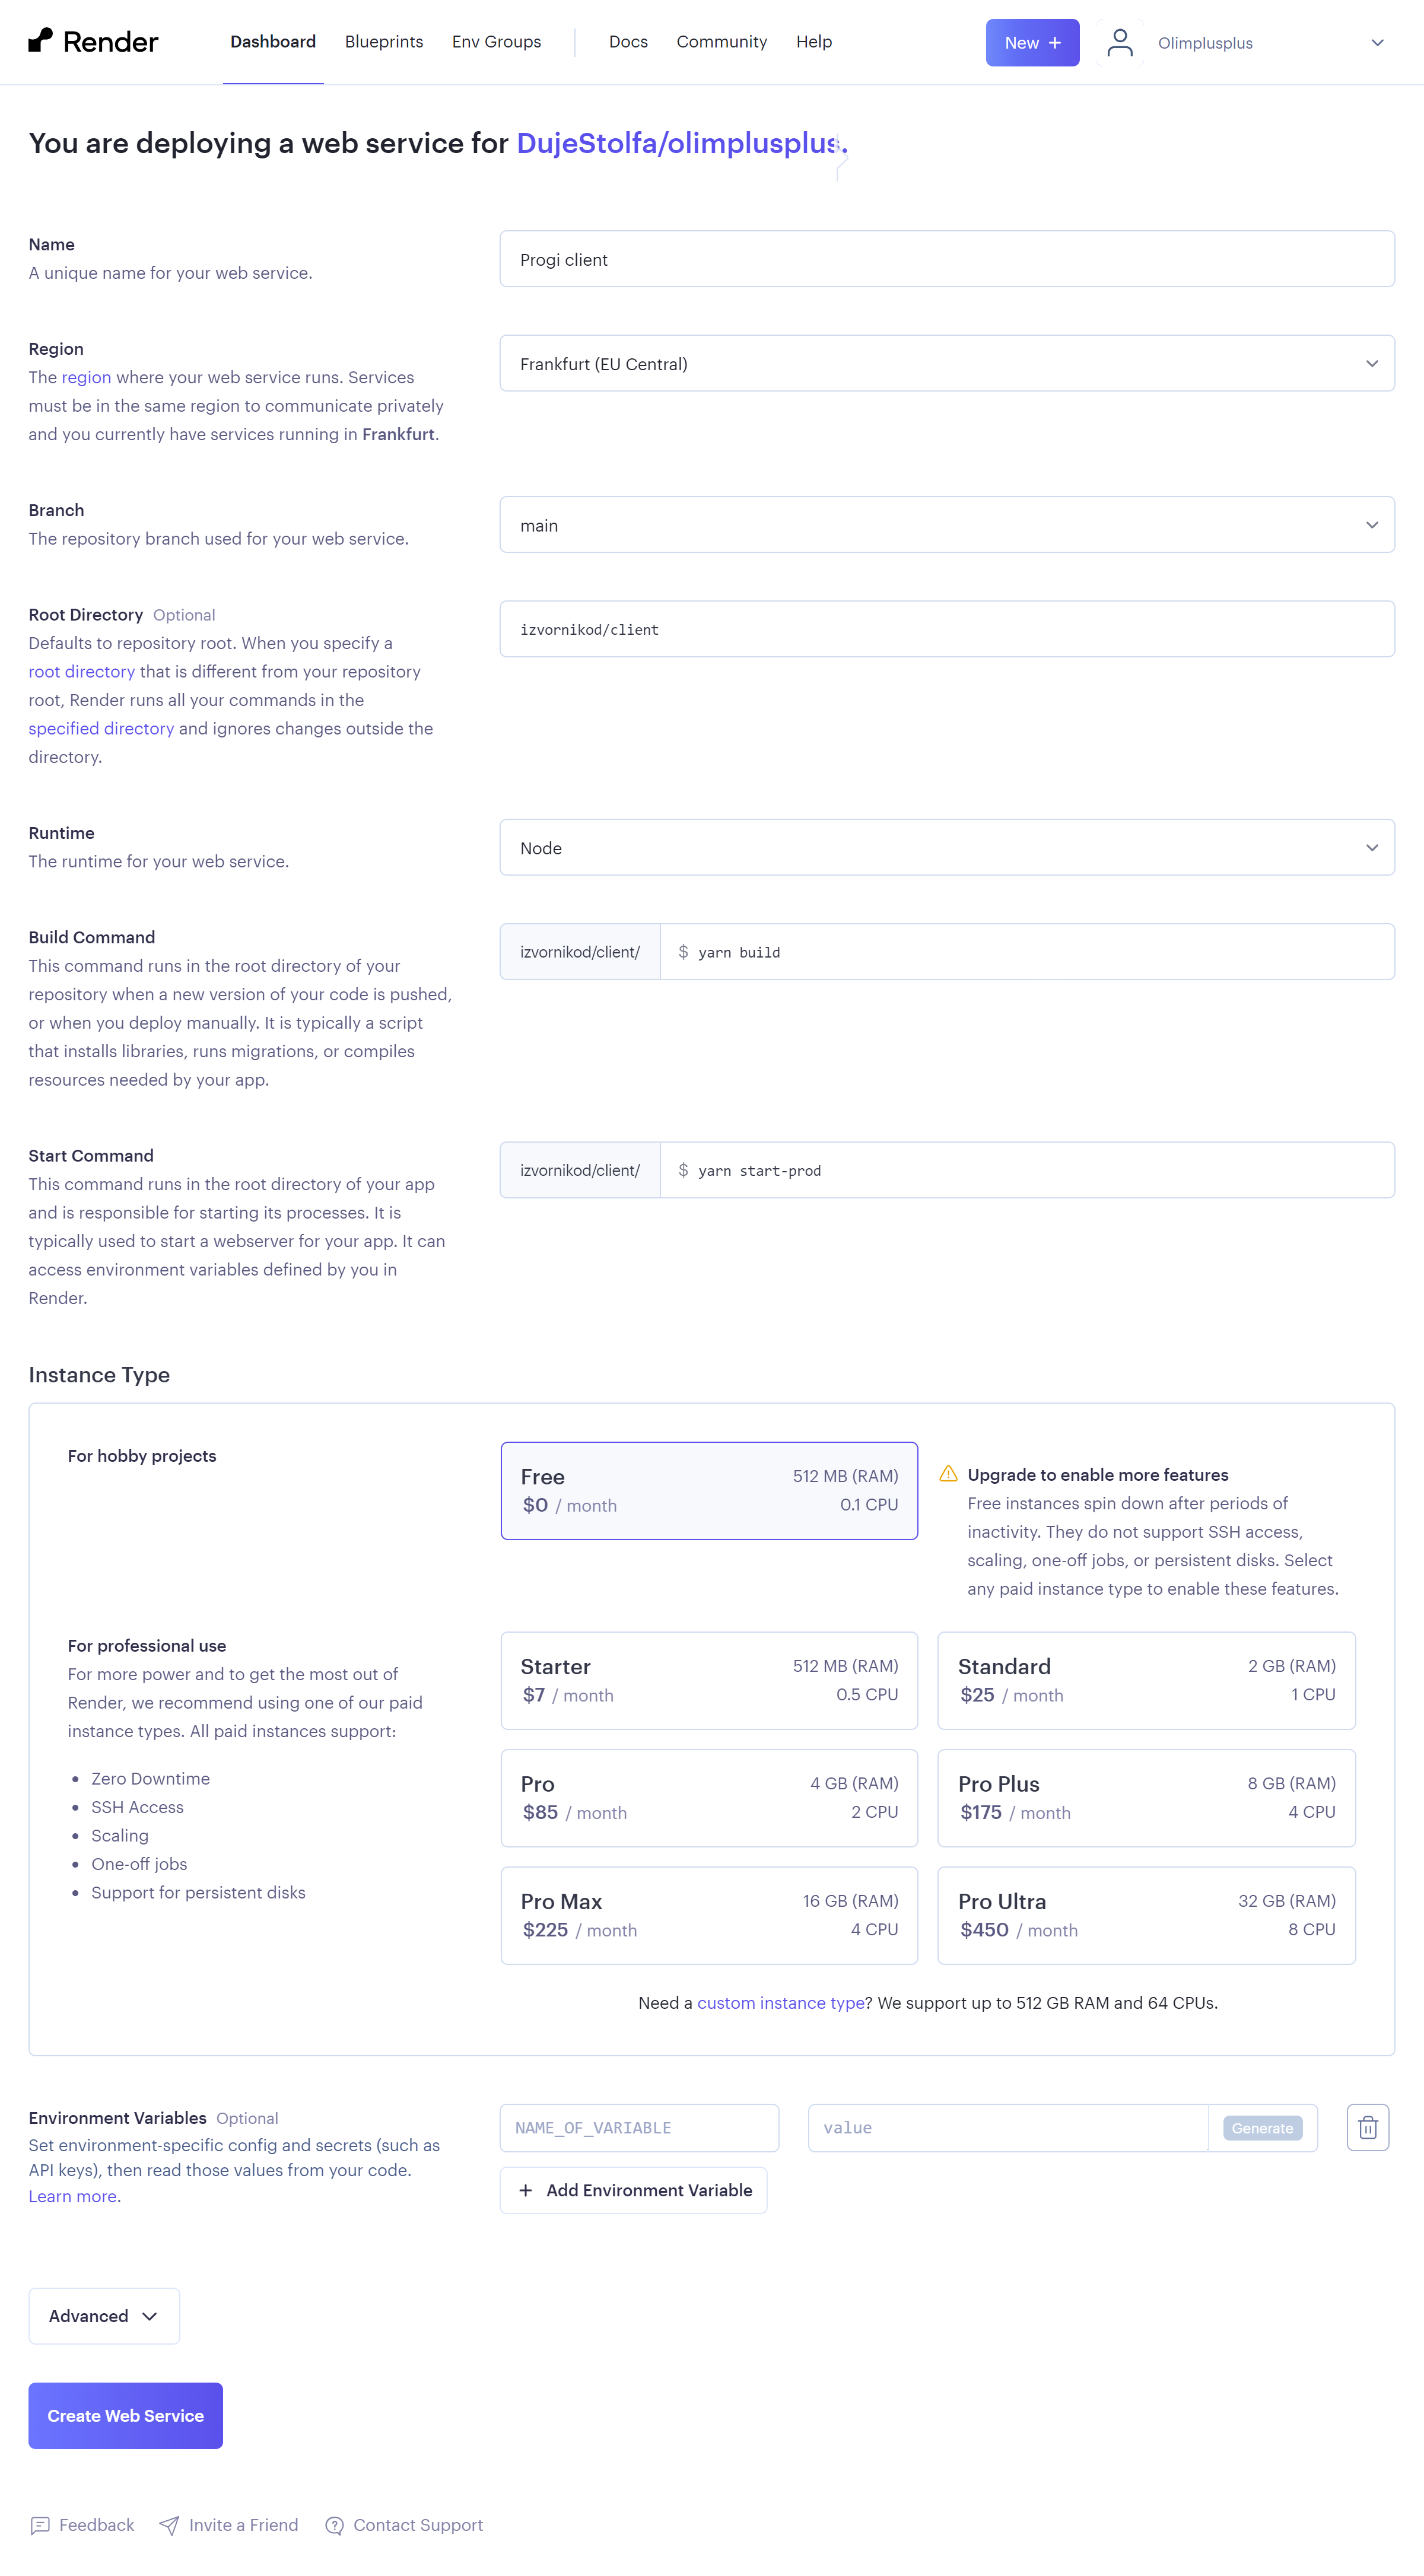
\includegraphics[scale=0.14]{slike/deploy_10.png}
			\centering
			\caption{Konfiguracija web servisa za frontend}
            \label{fig:dep-10}
		\end{figure}

        \begin{figure}[htp]
			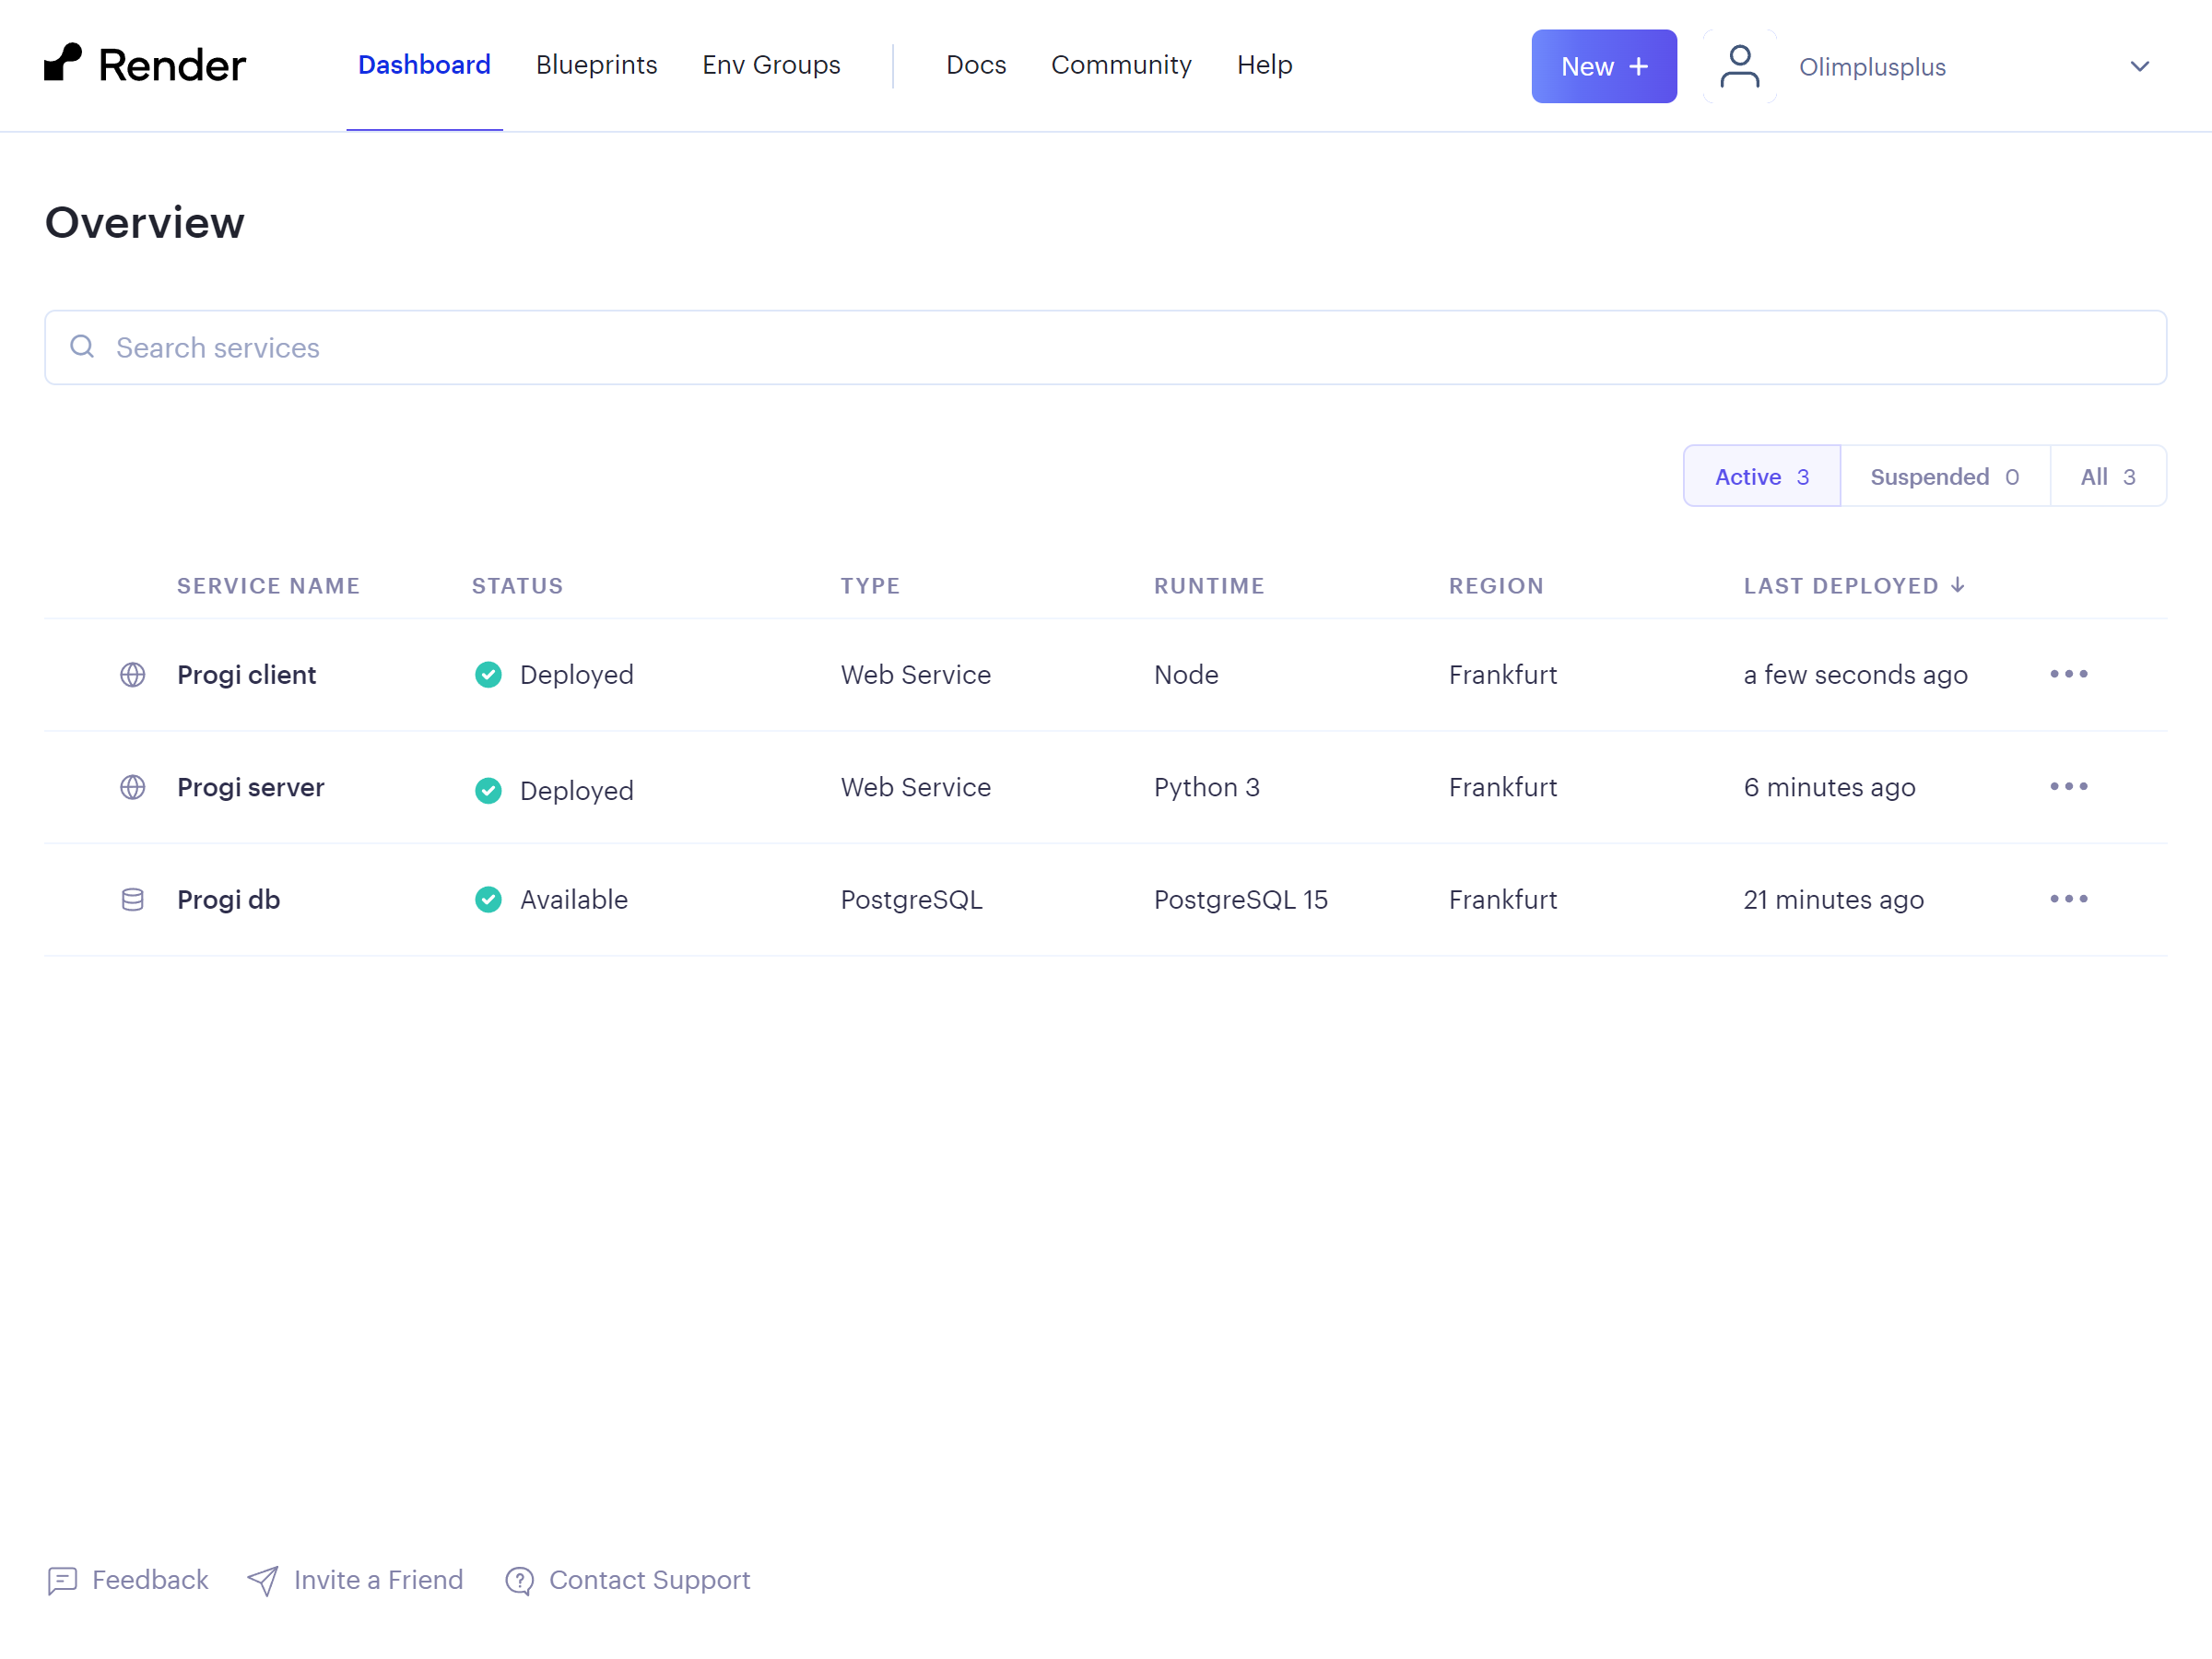
\includegraphics[scale=0.17]{slike/deploy_11.png}
			\centering
			\caption{Aktivne aplikacije u Renderu}
            \label{fig:dep-11}
		\end{figure}
			
			\eject 